\documentclass[12pt,twoside]{article}
%%%%%%%%%%%%%%%%%%%%%%%%%%%%%%%%%%%%%%%%%%%%%%%%%%%%%%%%%%%%%
% Meta informations:
\newcommand{\trauthor}{Sayantan Auddy}
\newcommand{\trtype}{Seminar Paper} %{Seminararbeit} %{Proseminararbeit}
\newcommand{\trcourse}{Independent Study}
\newcommand{\trtitle}{A Step Towards Bio-inspired Bipedal Locomotion}
\newcommand{\trmatrikelnummer}{6640595}
\newcommand{\tremail}{4auddy@informatik.uni-hamburg.de}
\newcommand{\trarbeitsbereich}{Knowledge Technology, WTM}
\newcommand{\trdate}{12.02.2017}
\newcommand{\suchthat}{\mid}

%%%%%%%%%%%%%%%%%%%%%%%%%%%%%%%%%%%%%%%%%%%%%%%%%%%%%%%%%%%%%
% Languages:

% Falls die Ausarbeitung in Deutsch erfolgt:
% \usepackage[german]{babel}
% \usepackage[T1]{fontenc}
% \usepackage[latin1]{inputenc}
% \usepackage[latin9]{inputenc}	 				
% \selectlanguage{german}

% If the thesis is written in English:
\usepackage[english]{babel} 						
\selectlanguage{english}

%%%%%%%%%%%%%%%%%%%%%%%%%%%%%%%%%%%%%%%%%%%%%%%%%%%%%%%%%%%%%
% Bind packages:
\usepackage{acronym}                    % Acronyms
\usepackage{algorithmic}				% Algorithms and Pseudocode
\usepackage{algorithm}					% Algorithms and Pseudocode
\usepackage{amsfonts}                   % AMS Math Packet (Fonts)
\usepackage{amsmath}                    % AMS Math Packet
\usepackage{amssymb}                    % Additional mathematical symbols
\usepackage{amsthm}
\usepackage{booktabs}                   % Nicer tables
%\usepackage[font=small,labelfont=bf]{caption} % Numbered captions for figures

\usepackage{color}                      % Enables defining of colors via \definecolor
\definecolor{uhhRed}{RGB}{254,0,0}      % Official Uni Hamburg Red
\definecolor{uhhGrey}{RGB}{122,122,120} % Official Uni Hamburg Grey
\usepackage{fancybox}                   % Gleichungen einrahmen
\usepackage{fancyhdr}					% Packet for nicer headers
%\usepackage{fancyheadings}             % Nicer numbering of headlines

%\usepackage[outer=3.35cm]{geometry} 	% Type area (size, margins...) !!!Release version
%\usepackage[outer=2.5cm]{geometry} 	% Type area (size, margins...) !!!Print version
%\usepackage{geometry} 					% Type area (size, margins...) !!!Proofread version
\usepackage[outer=3.15cm]{geometry} 	% Type area (size, margins...) !!!Draft version
\geometry{a4paper,body={5.8in,9in}}

\usepackage{graphicx}                   % Inclusion of graphics
%\usepackage{latexsym}                  % Special symbols
\usepackage{longtable}					% Allow tables over several pages
\usepackage{listings}                   % Nicer source code listings
\usepackage{multicol}					% Content of a table over several columns
\usepackage{multirow}					% Content of a table over several rows
\usepackage{rotating}					% Alows to rotate text and objects
\usepackage[hang]{subfigure}            % Allows to use multiple (partial) figures in a fig
%\usepackage[font=footnotesize,labelfont=rm]{subfig}	% Pictures in a floating environment
\usepackage{tabularx}					% Tables with fixed width but variable rows
\usepackage{url,xspace,boxedminipage}   % Accurate display of URLs
\usepackage{multirow}
\usepackage{tabulary}
\usepackage{float}


%%%%%%%%%%%%%%%%%%%%%%%%%%%%%%%%%%%%%%%%%%%%%%%%%%%%%%%%%%%%%
% Configurationen:

\hyphenation{whe-ther} 					% Manually use: "\-" in a word: Staats\-ver\-trag

%\lstloadlanguages{C}                   % Set the default language for listings
\DeclareGraphicsExtensions{.pdf,.svg,.jpg,.png,.eps} % first try pdf, then eps, png and jpg
\graphicspath{{./src/}} 				% Path to a folder where all pictures are located
\pagestyle{fancy} 						% Use nicer header and footer

% Redefine the environments for floating objects:
\setcounter{topnumber}{3}
\setcounter{bottomnumber}{2}
\setcounter{totalnumber}{4}
\renewcommand{\topfraction}{0.9} 		%Standard: 0.7
\renewcommand{\bottomfraction}{0.5}		%Standard: 0.3
\renewcommand{\textfraction}{0.1}		%Standard: 0.2
\renewcommand{\floatpagefraction}{0.8} 	%Standard: 0.5

% Tables with a nicer padding:
\renewcommand{\arraystretch}{1.2}

%%%%%%%%%%%%%%%%%%%%%%%%%%%%
% Additional 'theorem' and 'definition' blocks:
\theoremstyle{plain}
\newtheorem{theorem}{Theorem}[section]
%\newtheorem{theorem}{Satz}[section]	% Wenn in Deutsch geschrieben wird.
\newtheorem{axiom}{Axiom}[section] 	
%\newtheorem{axiom}{Fakt}[chapter]		% Wenn in Deutsch geschrieben wird.
%Usage:%\begin{axiom}[optional description]%Main part%\end{fakt}

\theoremstyle{definition}
\newtheorem{definition}{Definition}[section]

%Additional types of axioms:
\newtheorem{lemma}[axiom]{Lemma}
\newtheorem{observation}[axiom]{Observation}

%Additional types of definitions:
\theoremstyle{remark}
%\newtheorem{remark}[definition]{Bemerkung} % Wenn in Deutsch geschrieben wird.
\newtheorem{remark}[definition]{Remark} 

%%%%%%%%%%%%%%%%%%%%%%%%%%%%
% Provides TODOs within the margin:
\newcommand{\TODO}[1]{\marginpar{\emph{\small{{\bf TODO: } #1}}}}

%%%%%%%%%%%%%%%%%%%%%%%%%%%%
% Abbreviations and mathematical symbols
\newcommand{\modd}{\text{ mod }}
\newcommand{\RS}{\mathbb{R}}
\newcommand{\NS}{\mathbb{N}}
\newcommand{\ZS}{\mathbb{Z}}
\newcommand{\dnormal}{\mathit{N}}
\newcommand{\duniform}{\mathit{U}}

\newcommand{\erdos}{Erd\H{o}s}
\newcommand{\renyi}{-R\'{e}nyi}
\setlength{\parindent}{0pt}
\newcommand{\forceindent}{\leavevmode{\parindent=2em\indent}}
%%%%%%%%%%%%%%%%%%%%%%%%%%%%%%%%%%%%%%%%%%%%%%%%%%%%%%%%%%%%%
% Document:
\begin{document}
\renewcommand{\headheight}{14.5pt}

\fancyhead{}
\fancyhead[LE]{ \slshape \trauthor}
\fancyhead[LO]{}
\fancyhead[RE]{}
\fancyhead[RO]{ \slshape \trtitle}

%%%%%%%%%%%%%%%%%%%%%%%%%%%%
% Cover Header:
\begin{titlepage}
	\begin{flushleft}
		Universit\"at Hamburg\\
		Department Informatik\\
		\trarbeitsbereich\\
	\end{flushleft}
	\vspace{3.5cm}
	\begin{center}
		\huge \trtitle\\
	\end{center}
	\vspace{3.5cm}
	\begin{center}
		\normalsize\trtype\\
		[0.2cm]
		\Large\trcourse\\
		[1.5cm]
		\Large \trauthor\\
		[0.2cm]
		\normalsize Matr.Nr. \trmatrikelnummer\\
		[0.2cm]
		\normalsize\tremail\\
		[1.5cm]
		\Large \trdate
	\end{center}
	\vfill
\end{titlepage}

	%backsite of cover sheet is empty!
\thispagestyle{empty}
\hspace{1cm}
\newpage

%%%%%%%%%%%%%%%%%%%%%%%%%%%%
% Abstract:

% Abstract gives a brief summary of the main points of a paper:
\section*{Abstract}
The field of bipedal robots has advanced significantly over the last few decades. Yet even the most advanced robots cannot match the efficiency and gracefulness of human movement, which relies on a coordination between neural mechanisms and the dynamics of the skeletal structure. As an alternative to model based methods, Central Pattern Generators such as the Matsuoka oscillator  have emerged as a viable biologically inspired approach to achieve robust bipedal locomotion in robots. The use of the Matsuoka oscillator on position controlled robots is limited by the fact that this oscillator generates torques and is more suitable for torque controlled robots. In this paper, a novel way to overcome this problem is presented. This technique can be extended in the future into a framework that can lead to robust walking and is not tightly coupled to a particular robot model.

% Lists:
\setcounter{tocdepth}{2} 					% depth of the table of contents (for Seminars 2 is recommented)
\tableofcontents
\pagenumbering{arabic}
\clearpage

%%%%%%%%%%%%%%%%%%%%%%%%%%%%
% Content:

% the actual content, usually separated over a number of sections
% each section is assigned a label, in order to be able to put a
% crossreference to it

\graphicspath{{images/}}

\section{Introduction}
\label{sec:introduction}
Walking on two feet is an activity that all of us take for granted. Yet this apparently simple action involves a host of complex mechanisms which are tied together to produce the bipedal movements of human beings. The ability to move around on two legs has allowed humans to effectively deal with a wide variety of terrains. The efficiency and versatility of biped movement is undeniable, and so it is natural for us to desire our robots to have the same capabilities.\\
\forceindent However, the benefits of legged robots comes at a price. Bipedal locomotion is inherently unstable, and a considerable amount of effort goes into maintaining balance. In addition, it involves a complicated mix of  movements of different limbs in a synchronous fashion. Human walking involves multiple degrees of freedom and is achieved with the combined effort of muscles, bones, ligaments and tendons. Replicating this movement in robots using the conventional servo motors we have at our disposal today, is also a very difficult task.\\
\forceindent In the literature, perhaps the most popular approach for solving the problem of bipedal movement is that of using the  Zero Moment Point (ZMP) \cite{vukobratovic1969contribution, jurivcic1972mathematical}. ZMP is defined as that point on the ground at which the net moment of the inertial forces and the gravity forces has no component along the horizontal axes \cite{vukobratovic2004zero}. By ensuring that the ZMP always lies within the support polygon of the robot, dynamical stability of the system can be ensured. The approach then is to find a suitable trajectory of the ZMP and then to use inverse kinematics to figure out what the individual joint angle trajectories should be which satisfy the required ZMP trajectory.\\
\forceindent However despite the popularity of ZMP, it has some limitations. Firstly, the computation of ZMP and the subsequent computation of joint angle trajectories is computationally intensive and depends on an accurate model of the robot. Secondly, such robots move in a very conservative manner with bent knees and slow carefully placed steps. In this sense, the movement of ZMP based robots is very different from the movement of humans, which is characterized by almost straight knees and fast steps. Animals are adept at utilizing the passive dynamics of their bodies for walking. This leads to an energy efficient mode of transport. ZMP based robots, on the other hand, cancel out the natural dynamics of the mechanical system in an effort to maintain control over the system at all times, and this leads to high energy consumption.\\
\forceindent As with so many other areas of robotics, for walking too, we can draw inspiration from nature and build systems that try to emulate the mechanisms present in animals. This is the approach followed in this paper, where a neural mechanism known as Central Pattern Generators (CPG) is utilized for controlling robot joints. This technique can be extended into a framework for bipedal locomotion. The remainder of this paper is organized as follows. In section \ref{sec:Related_Work}, some relevant work is discussed. This is followed in section \ref{sec:Biological_Motivation} by a discussion of the neural mechanisms of walking. The advantages of the Matsuoka oscillator over other oscillators is discussed in section \ref{sec:Choice_of_Oscillator}.  Section \ref{sec:Matsuoka_Oscillator} contains an in-depth discussion of the Matsuoka oscillator and its properties. This is followed by section \ref{sec:Robot_Joint_Control}, where a novel process of using an oscillator to control a position controlled robot joint is described. Section \ref{sec:Future_Work} describes how this technique of joint control can be extended into a framework of bipedal locomotion. Finally section \ref{sec:Conclusion} contains concluding remarks about the work presented in this paper.



\section{Related Work}
\label{sec:Related_Work}
Research on bipedal locomotion has yielded a number of  ways in which humanoid robots can be made to walk in a stable manner. In \cite{kajita2003biped} Kajita et al. have presented a method to generate ZMP and Center of Mass (CoM) trajectories of the robot using a technique known as preview control, where the reference ZMP is known for a few seconds into the future. In \cite{kajita2010biped} Kajita et al. achieved stabilization using the Linear Inverted Pendulum (LIP) model on a 42-degree-of-freedom (DoF) adult sized humanoid robot. In \cite{kajita20013d} the authors have presented a simplified model (3D-LIP) which can be used to accurately model the dynamics of a high DoF robot.\\
\forceindent An argument against pure ZMP based methods, put forward by Missura et al. in \cite{missura2013omnidirectional, missura2014online, missura2015gradient}, is that such methods are not suitable in situations where the robot may be subject to strong disturbances. The authors have presented a hierarchical gait control architecture where balance control is separated from motion generation. This architecture relies on the LIP model and is able to resist strong disturbances using a combination of different strategies including ZMP. In \cite{stephens2007humanoid}, simple models for humanoids have been investigated with respect to push recovery.\\
\forceindent However, despite the popularity of ZMP based techniques, the gait of even highly sophisticated humanoid robots such as ASIMO is very different from the gait of humans. An interesting alternative to the computationally involved ZMP technique is that of passive walking. McGeer's work \cite{mcgeer1990passive} has shown that highly efficient human-like gait can be achieved even by an unactuated humanoid walking down a ramp. McGeer's passive walkers have highlighted the fact that if the physical constraints of the robot can be utilized efficiently, then human-like motion is achievable without relying on excessively complicated techniques.\\
\forceindent While passive walking relies on exploiting the mechanical constraints of the robot's structure, on its own it cannot yield walkers which can tackle different terrains, slopes or situations. To do this a controller is required which can utilize information from the robot's external and proprioceptive sensors to adapt the gait as required. In \cite{geng2005fast} a neural network controlled biped walker has been presented. A reflexive hierarchical controller controls biped walking without any kind of trajectory control. Reinforcement learning has been used to tune the parameters of the controller. In \cite{paul2005sensorimotor} sensorimotor neural networks (one for each leg) control the motion of the biped. The network is optimized using a genetic algorithm.\\
\forceindent Taking the biological inspiration factor a step further, Central Pattern Generators have been used to design the low level neural circuitry that controls bipedal locomotion. CPGs are biological neural networks which produce rhythmic output on their own without the need of any sensory feedback. The output of the individual networks control the movement of the individual limbs and can be modulated using sensory feedback to produce different kinds of motion. Typically the parameters of the CPG are tuned using some kind of evolutionary algorithm. Various mathematical models, known as oscillators, are available which encapsulate the behavior of the CPG in the form of coupled non-linear differential equations. The most used oscillators are the Van der Pol oscillator \cite{kanamaru2007van}, the Hopf oscillator \cite{Righetti2006} and the Matsuoka oscillator \cite{Matsuoka1985,Matsuoka1987}. In \cite{Righetti2006} and \cite{Kieboom2009}, Hopf oscillators have been used for pattern generation, along with some feedback mechanisms for stabilizations. Taga \cite{Taga1991} produced the seminal work in which Matsuoka oscillators were used for gait generation of a two dimensional planar biped robot. Ishiguro et al. \cite{Ishiguro2003} have presented an approach in which a CPG circuit is modulated using simulated neuromodulators to achieve stable bipedal locomotion. In \cite{Ijspeert2008} Ijspeert has provided a comprehensive review of the use of CPGs for locomotion control.

\section{Biological Motivation}
\label{sec:Biological_Motivation}
In both higher level vertebrates such as humans as well as in invertebrates, neural circuits known as Central Pattern Generators are responsible for producing the rhythmic movements which are responsible for locomotion \cite{Ijspeert2008}. These CPGs can produce rhythmic patterns of neural activity without the need of rhythmic or sensory inputs, and they are the basis of fundamental activities such as chewing, breathing and locomotion. Several studies have proven the existence of CPGs in animals and their responsibility for the movements of the animals \cite{cohen1980neuronal,grillner1985neural,stein1999neurons}. Although sensory feedback is not required to generate the rhythmic patterns by CPGs, it plays an important role in modulating the rhythmic patterns \cite{Ijspeert2008}. Vertebrate locomotor systems are organized such that the CPGs produce basic rhythmic patterns, and the higher brain centres modulate these patterns based on external sensory inputs \cite{Ijspeert2008}. Such an organization has important consequences, even from a robotics perspective, since it drastically reduces the dimensionality of higher level control signals. The higher centres do not need to specify individual muscle (or joint) activity and instead only need to modulate the CPG activity using a small set of parameters.\\
\forceindent A general framework for the nervous control of motor systems is illustrated in figure \ref{fig:neural_comp}. The first element in this framework is the CPG, located in the spinal cord \cite{neurobiology1994shepherd}. This is responsible for generating coordinated rhythmic outputs for the motor neurons. The CPG in turn is controlled and modulated by the higher motor centres. There also exist feedback circuits which relay information from the muscles (proprioceptive feedback) and from the environment through other sensory pathways \cite{neurobiology1994shepherd}. The feedback information is transmitted from lower to higher centres. The proprioceptive feedback informs the higher center about any deviations that exist between the commanded signal and the output \cite{neurobiology1994shepherd}.

\begin{figure}[htbp]
\centering     %%% not \center
\subfigure[Neural components of motor systems. Feedback information flows from the lower centers to the higher centers. Sensory input to CPG is only used for modulation. The CPGs can produce rhythmic output in the absence of sensory input as well \cite{neurobiology1994shepherd}]{\label{fig:neural_comp}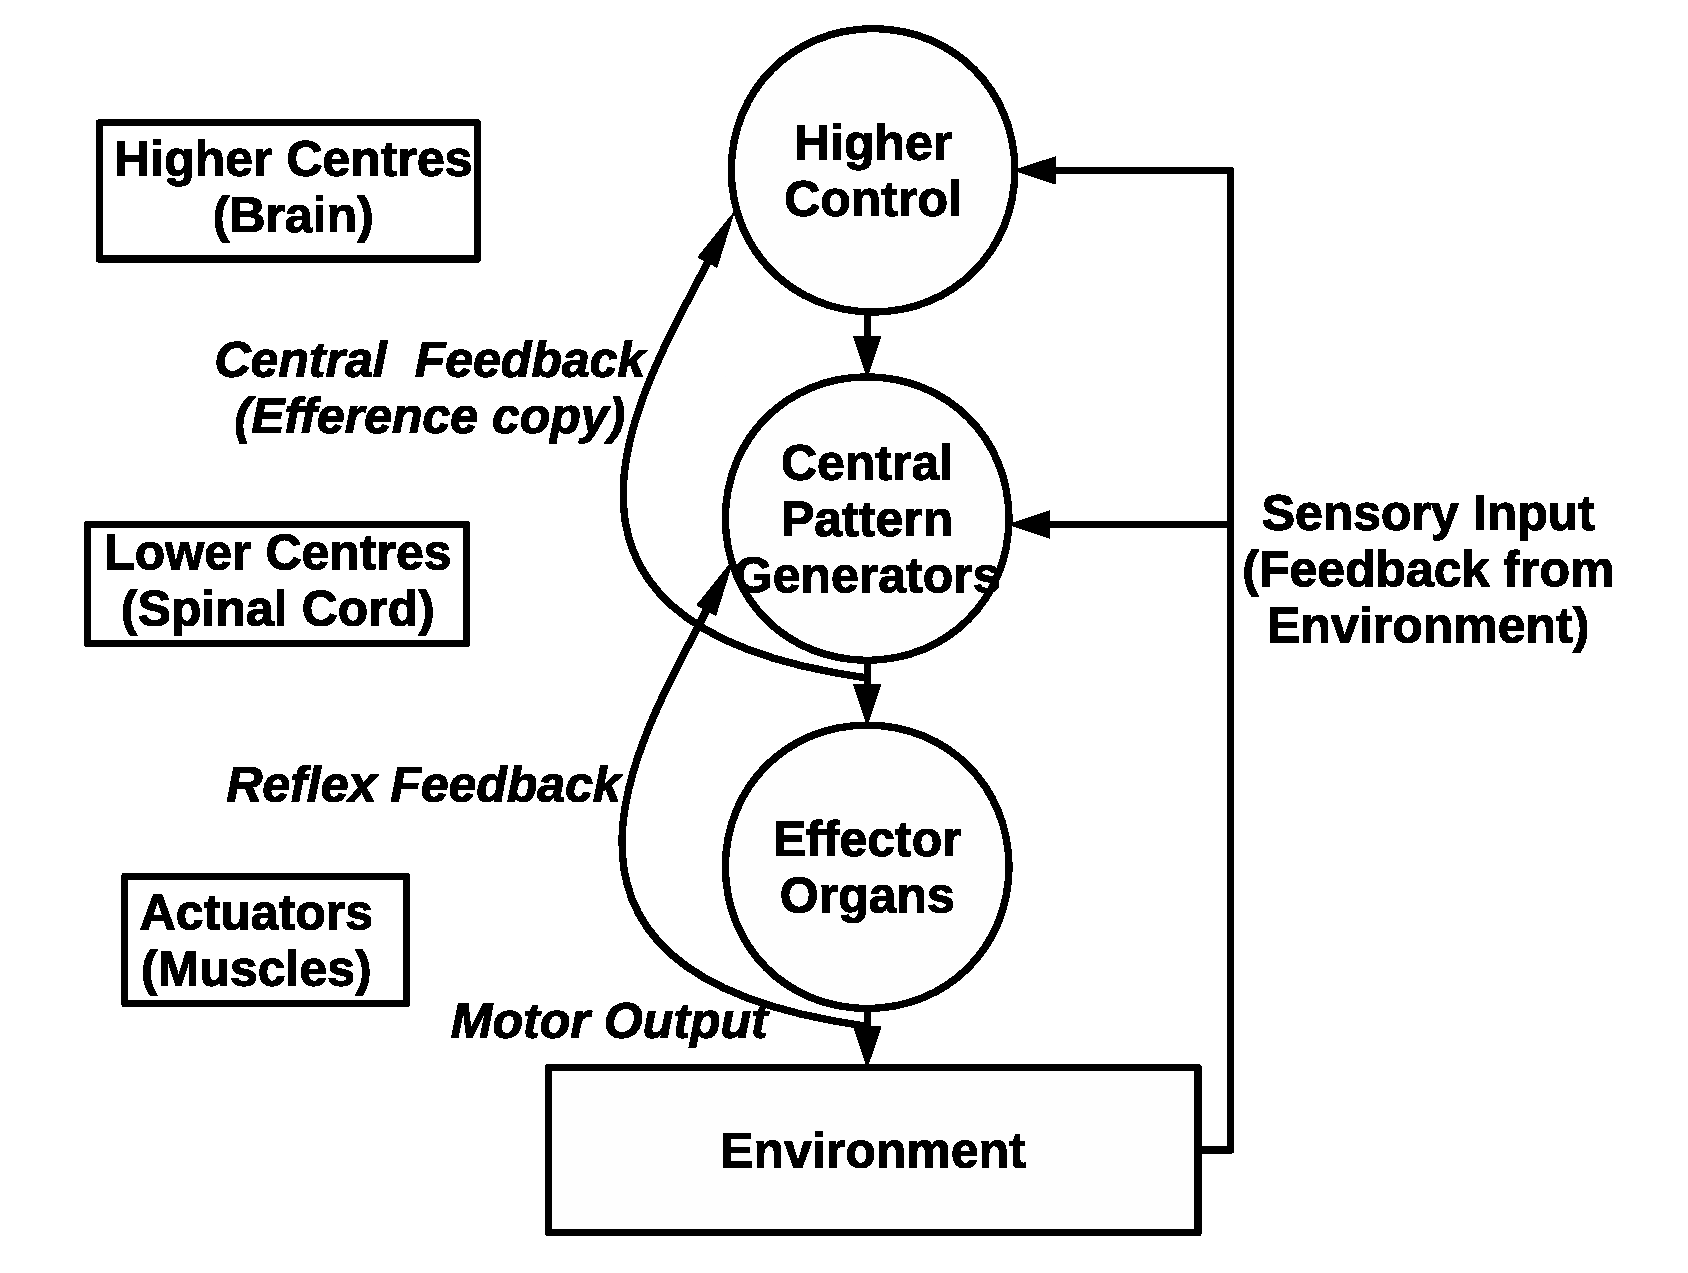
\includegraphics[scale=0.26]{figures/neural_comp.eps}}
\subfigure[Half-center model. D denotes driver neurons which supply a constant input, E and F are the extensor and flexor motor neurons. Filled profiles indicate inhibitory neurons, open profiles denote excitatory neurons \cite{neurobiology1994shepherd}]{\label{fig:half_center}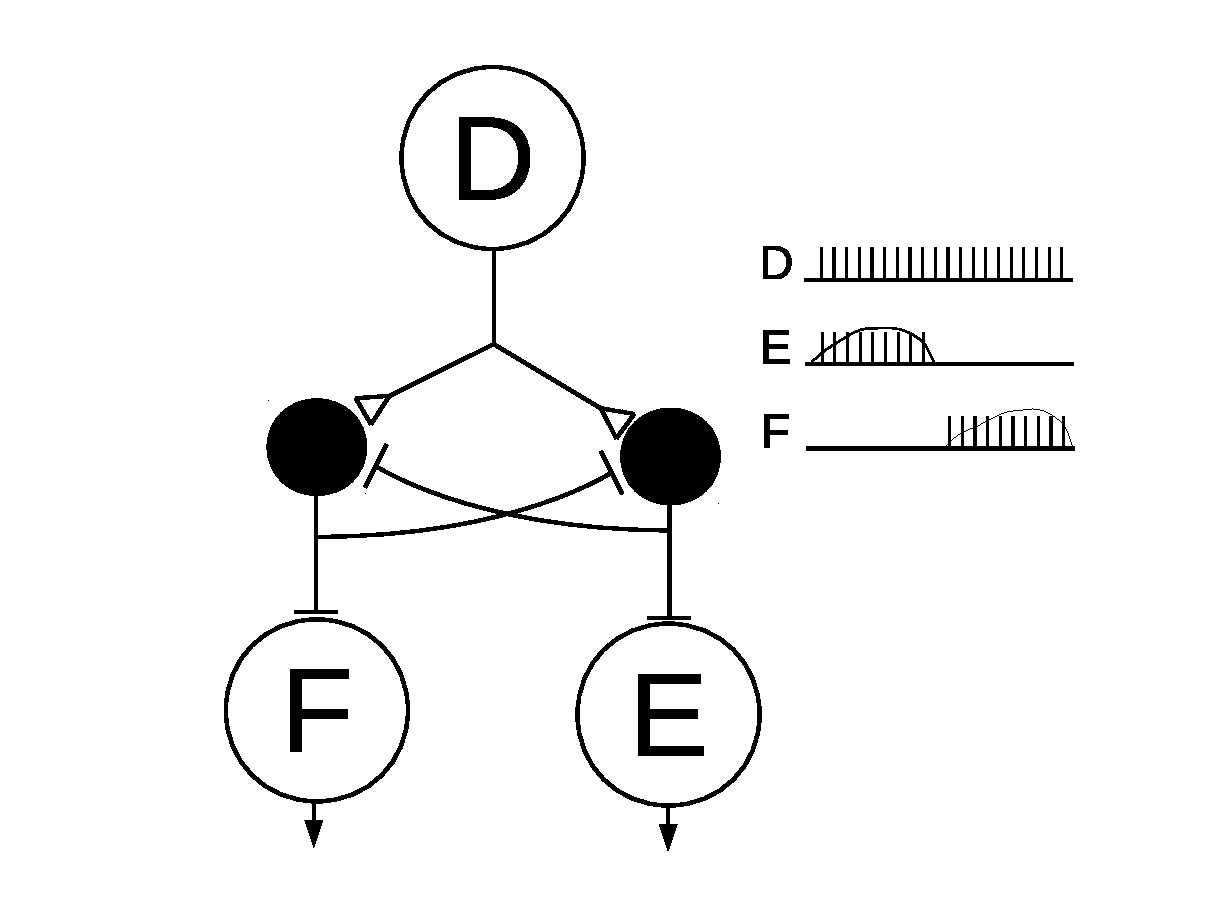
\includegraphics[scale=0.2]{figures/half_center_model.eps}}
\caption{Neural components of motor systems and a half-center CPG model \cite{neurobiology1994shepherd}}
\end{figure}

\forceindent The internal circuitry of the CPG generally belongs to one of three major categories: the half-center model, the closed-loop model and the pacemaker model \cite{neurobiology1994shepherd}. Only the half-center model is discussed here as it is relevant to the material in the subsequent sections. The half-center model, as shown in figure \ref{fig:half_center}, was first proposed by Brown \cite{brown1914nature} to explain the alternating activation of the flexor and extensor muscles of a decerebrated cat's limbs during walking on a treadmill. Each pool of motor neurons for flexor (F) or extensor (E) is activated by a corresponding half-center of interneurons. Another set of neurons (D) provides a constant excitatory drive to the half-centres. Each half-center has inhibitory connections to the other half-center, and this ensures that when one pool is activated, the other one is deactivated. According to Brown, as the first half-center was activated, a process of fatigue would build up in the inhibitory connection between the half-centres which would ultimately lead to a switching of activity between the half-centres. The process of fatigue can be modelled by any process that induces self-inhibition of the active half-centres \cite{neurobiology1994shepherd}.\\
\forceindent The inherent properties of CPGs make them a suitable candidate for the locomotion control of legged robots, as opposed to controllers based on ZMP \cite{Ijspeert2008}. First of all, CPG based models display stable limit cycle behavior, which means that although the generated patterns may be modified under the effect of a disturbance, as soon as the disturbance is removed, the CPG returns to its normal behavior. This property maybe beneficial in situations where robots need to tackle uneven terrain. Secondly, CPG based controllers have very few parameters and hence higher level controllers need not deal with low level motor commands. Thirdly, CPGs can handle sensory feedback easily, since the feedback signals can be conveniently added as coupling terms in the differential equations. This also leads to the property of entrainment, where the CPG tunes itself to the dynamics of the mechanical system and can effectively utilize the dynamics of the robot \cite{Ijspeert2008}.


\section{Choice of Oscillator}
\label{sec:Choice_of_Oscillator}
In bipedal locomotion research, the most used oscillators are the Hopf oscillator and the Matsuoka oscillator. The Hopf oscillator has been used successfully by Righetti and Ijspeert \cite{Righetti2006} and by Kieboom \cite{Kieboom2009} to design controllers for a bipedal robot. Matsuoka oscillators have also been used for the same purpose by Taga \cite{Taga1991}, Ishiguro et al. \cite{Ishiguro2003} and by Cristiano et al. \cite{cristiano2014locomotion}. The Hopf oscillator is well defined in terms of amplitude and frequency, is easy to control and has strong limit cycle properties \cite{Kieboom2009}. Moreover, different oscillators maybe easily combined to produce complex output patterns \cite{Righetti2006}. \\
\forceindent However, one disadvantage is that the Hopf oscillator needs an appropriate teaching signal to which the oscillator entrains to produce a suitable pattern. In \cite{Righetti2006}, the authors have used the joint angle patterns produced by the manufacturer-provided walking algorithm as the teaching signal to train the oscillator network. The problem with this approach is that the CPG based walking algorithm will produce the same gait as the default algorithm, and will replicate the deficiencies of that algorithm. For a new robot, a default walking algorithm may not be  available. In \cite{Kieboom2009}, the author has used a system of optimized sine generators as the teaching signal for a network of Hopf oscillators. Here additional effort is spent in optimizing the sine equation parameters, and again the teaching signals themselves are very simple and cannot efficiently utilize the robot's dynamics to their advantage.\\
\forceindent The Matsuoka oscillator does not need a teaching signal, can be optimized in a single step to generate waveforms of a desired nature and can be entrained with the mechanics of the biped in an automatic sense \cite{Kieboom2009}. Additionally, among the different oscillators, Matsuoka oscillators are the most plausible biologically and the two-neuron Matsuoka oscillator \cite{Matsuoka1987} bears a very close resemblance to the half-center model described in section \ref{sec:Biological_Motivation}. Keeping in mind the relative advantages of the Matsuoka oscillator over the Hopf oscillator, it has been chosen as the oscillator model for implementing the CPGs in this paper.


\section{Matsuoka Oscillator}
\label{sec:Matsuoka_Oscillator}
The Matsuoka oscillator is a mathematical model representing a general class of neural rhythm generators called mutual inhibition networks \cite{Matsuoka1987}. In this oscillator a set of neurons inhibit each others activities. For the individual neurons, a continuous-time continuous-variable neuron model is adopted \cite{Matsuoka1987}. The autonomous dynamics of the model are based on a piece-wise linear set of differential equations which model the dynamics of neural discharge rates. The oscillator consists of a pair of neurons whose rates of discharge are denoted by $\psi_i$ and $\psi_j$ respectively. The firing rates obey the following equations \cite{Ronsse2009}: 
\begin{subequations} 
\label{eq:matsuoka_basic}
\begin{align}
 t_1 \dot{\psi_i}=-\psi_i - \beta \phi_i - \eta [\psi_j]^+ + u_i\\
 t_1 \dot{\psi_j}=-\psi_j - \beta \phi_j - \eta [\psi_i]^+ + u_j
 \end{align}
\end{subequations}
where $t_1$ is the time constant for the rate of discharge, $\beta$ is the self-inhibition constant and $\eta$ is the constant of mutual inhibition. $u_i$ and $u_j$ denote the constant (tonic) input signals that drive the oscillator. $\phi_i$ and $\phi_j$ are state variables which control the self-inhibition. $[\textbf{\textbullet}]^+=max(0,\textbf{\textbullet})$ implies that only the positive part of the discharge rates is considered for mutual inhibition. Equation  \ref{eq:matsuoka_basic} can be further extended by including terms representing the proprioceptive feedback, which will enable the system to monitor and rectify errors between the commanded and executed trajectories. A way of doing this was suggested in \cite{Williamson1998}, by including the sensory feedback into the firing rate equations (equation \ref{eq:matsuoka_basic}). On doing so these equations are modified into:
\begin{subequations} 
\label{eq:matsuoka_extended}
\begin{align}
 t_1 \dot{\psi_i}=-\psi_i - \beta \phi_i - \eta [\psi_j]^+ - \sigma [\theta - \theta^{*}] + u_i\\
 t_1 \dot{\psi_j}=-\psi_j - \beta \phi_j - \eta [\psi_i]^+ - \sigma [-(\theta - \theta^{*})] + u_j
 \end{align}
\end{subequations}
Here, $\sigma$ is the strength of the sensory feedback, $\theta$ denotes the proprioceptive feedback and $\theta^{*}$ denotes the desired reference output angle (the mean position about which oscillations should occur). It should be kept in mind that this sensory feedback is not required for producing oscillations but only to make sure that the oscillations occur about a reference position. The state variables $\phi_i$ and $\phi_j$ obey the following equations \cite{Ronsse2009}: 
\begin{subequations} 
\label{eq:matsuoka_phi}
\begin{align}
 t_2 \dot{\phi_i}=-\phi_i + [\psi_i]^+\\
 t_2 \dot{\phi_j}=-\phi_j + [\psi_j]^+
 \end{align}
\end{subequations}
Here, $t_2$ is the time constant of adaptation or fatigue. The time constants $t_1$ and $t_2$ play an important role in the generation of oscillations. The discharge of a neuron with a constant input $u$ will first rise to a maximum value in a time governed by $t_1$ and then gradually decrease to a lower value in a time governed by $t_2$. Robust oscillations emerge due to a balance between self-inhibition and mutual-inhibition. The discharge rates $\psi_i$ and $\psi_j$ are assumed to be proportional to the torque generated in the positive and negative directions respectively \cite{Ronsse2009}. Hence the net torque is given by: 
\begin{equation}
\label{eq:matsuoka_net_torque}
\psi_T=h_{\psi}([\psi_i]^+ - [\psi_j]^+)
\end{equation}
where $h_{\psi}$ is the gain factor. The resultant torque can be converted into the desired joint velocity $\dot{\theta}$ and angular position $\theta$ by solving the following differential equation of a simple inertial mechanical system \cite{Ronsse2009}:
\begin{equation}
\label{eq:inertial_system}
I\ddot{\theta} + \gamma \dot{\theta} - \psi_T = 0
\end{equation}
Here, $I$ is the moment of inertia and $\gamma$ is the damping constant. A pictorial representation of a Matsuoka oscillator driving a single joint (with proprioceptive feedback) is shown in figure \ref{fig:matsuoka_diagram}.

\begin{figure}[hbtp]
  \begin{minipage}[c]{0.45\textwidth}
    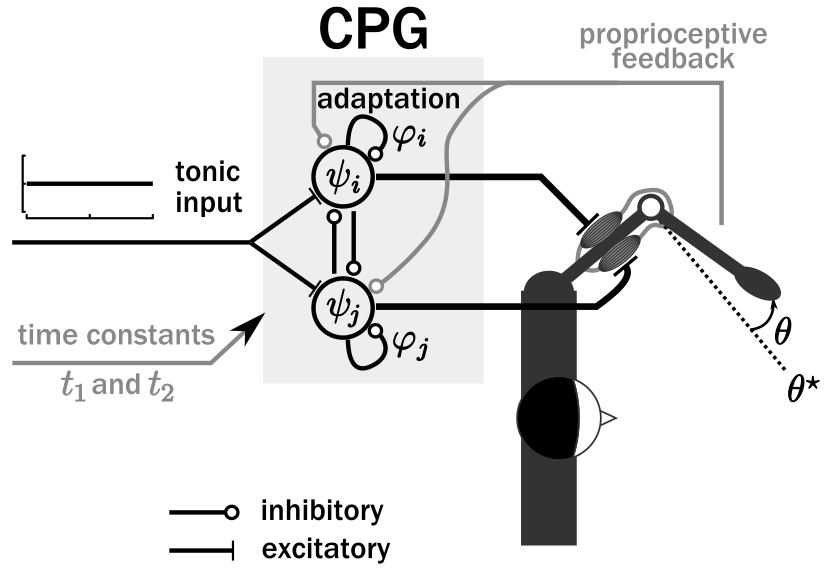
\includegraphics[width=\textwidth]{figures/matsuoka_diagram.png}
  \end{minipage}\hfill
  \begin{minipage}[c]{0.4\textwidth}
    \caption{Matsuoka oscillator driving two antagonistic muscles. The difference of the torques produced by the two neurons is the net torque that drives the joint. Proprioceptive feedback is denoted by the gray line. Lines with empty circles at the end denote inhibitory connections \cite{Ronsse2009}.
        } \label{fig:matsuoka_diagram}
  \end{minipage}
\end{figure}

\forceindent Since the basic equations of the Matsuoka oscillator are now in place, it is worthwhile to investigate how the parameters of the oscillator affect the output pattern. This will lead to a better understanding of how to achieve desired movements of the robot by changing oscillator parameters. According to equations \ref{eq:matsuoka_basic}-\ref{eq:matsuoka_net_torque}, the oscillator parameters are $t_1$ (time constant for the rate of discharge), $t_2$ (time constant of fatigue), $\beta$ (self-inhibition constant), $\eta$ (mutual-inhibition constant), $u_i$, $u_j$ (tonic inputs, $u_i=u_j$) , $\sigma$ (strength of sensory feedback),  $\theta^*$ (desired reference angular position) and $h_{\psi}$ (torque gain). $\psi_i$, $\psi_j$, $\phi_i$, $\phi_j$ are the state variables. In each of the three examples below, one parameter is modulated while the others are kept constant. The constant parameters are $t_1=0.25$, $t_2= 2.5 \times t_1$ as per \cite{Ronsse2009}, $\beta=2.5$,  $\eta=2.5$, $u_i=u_j=1$, $\sigma=1.5$, $\theta^*=0$ and $h_{\psi}=5.0$. The modulated parameter and its value are mentioned for each example.\\ 

\forceindent First the effect of changing the desired reference position on the angular trajectory is demonstrated. On its own, the Matsuoka oscillator produces oscillations about an arbitrary position, and the system itself is dynamically unstable. However, with the introduction of a feedback term (equation \ref{eq:matsuoka_extended}) and by modulating the parameter $\theta^*$, the mean position of oscillations can be controlled \cite{Ronsse2009} (figure \ref{fig:change-avg-pos}). For the first 10 seconds $\theta^*=0$ radians, from 10-20s, $\theta^*=1$ radian and from 20-30s $\theta^*=-1$ radian. As illustrated by the joint position graph (figure \ref{fig:change-avg-pos-b}), the mean oscillation position changes and the transition is smooth.  This kind of situation maybe encountered when the robot initially moves on a flat surface and then steps upon an inclined surface. At this point the mean oscillation position of some joints would change.

\begin{figure}[hbtp]
\centering     %%% not \center
\subfigure[Torque output of the oscillator]{\label{fig:change-avg-pos-a}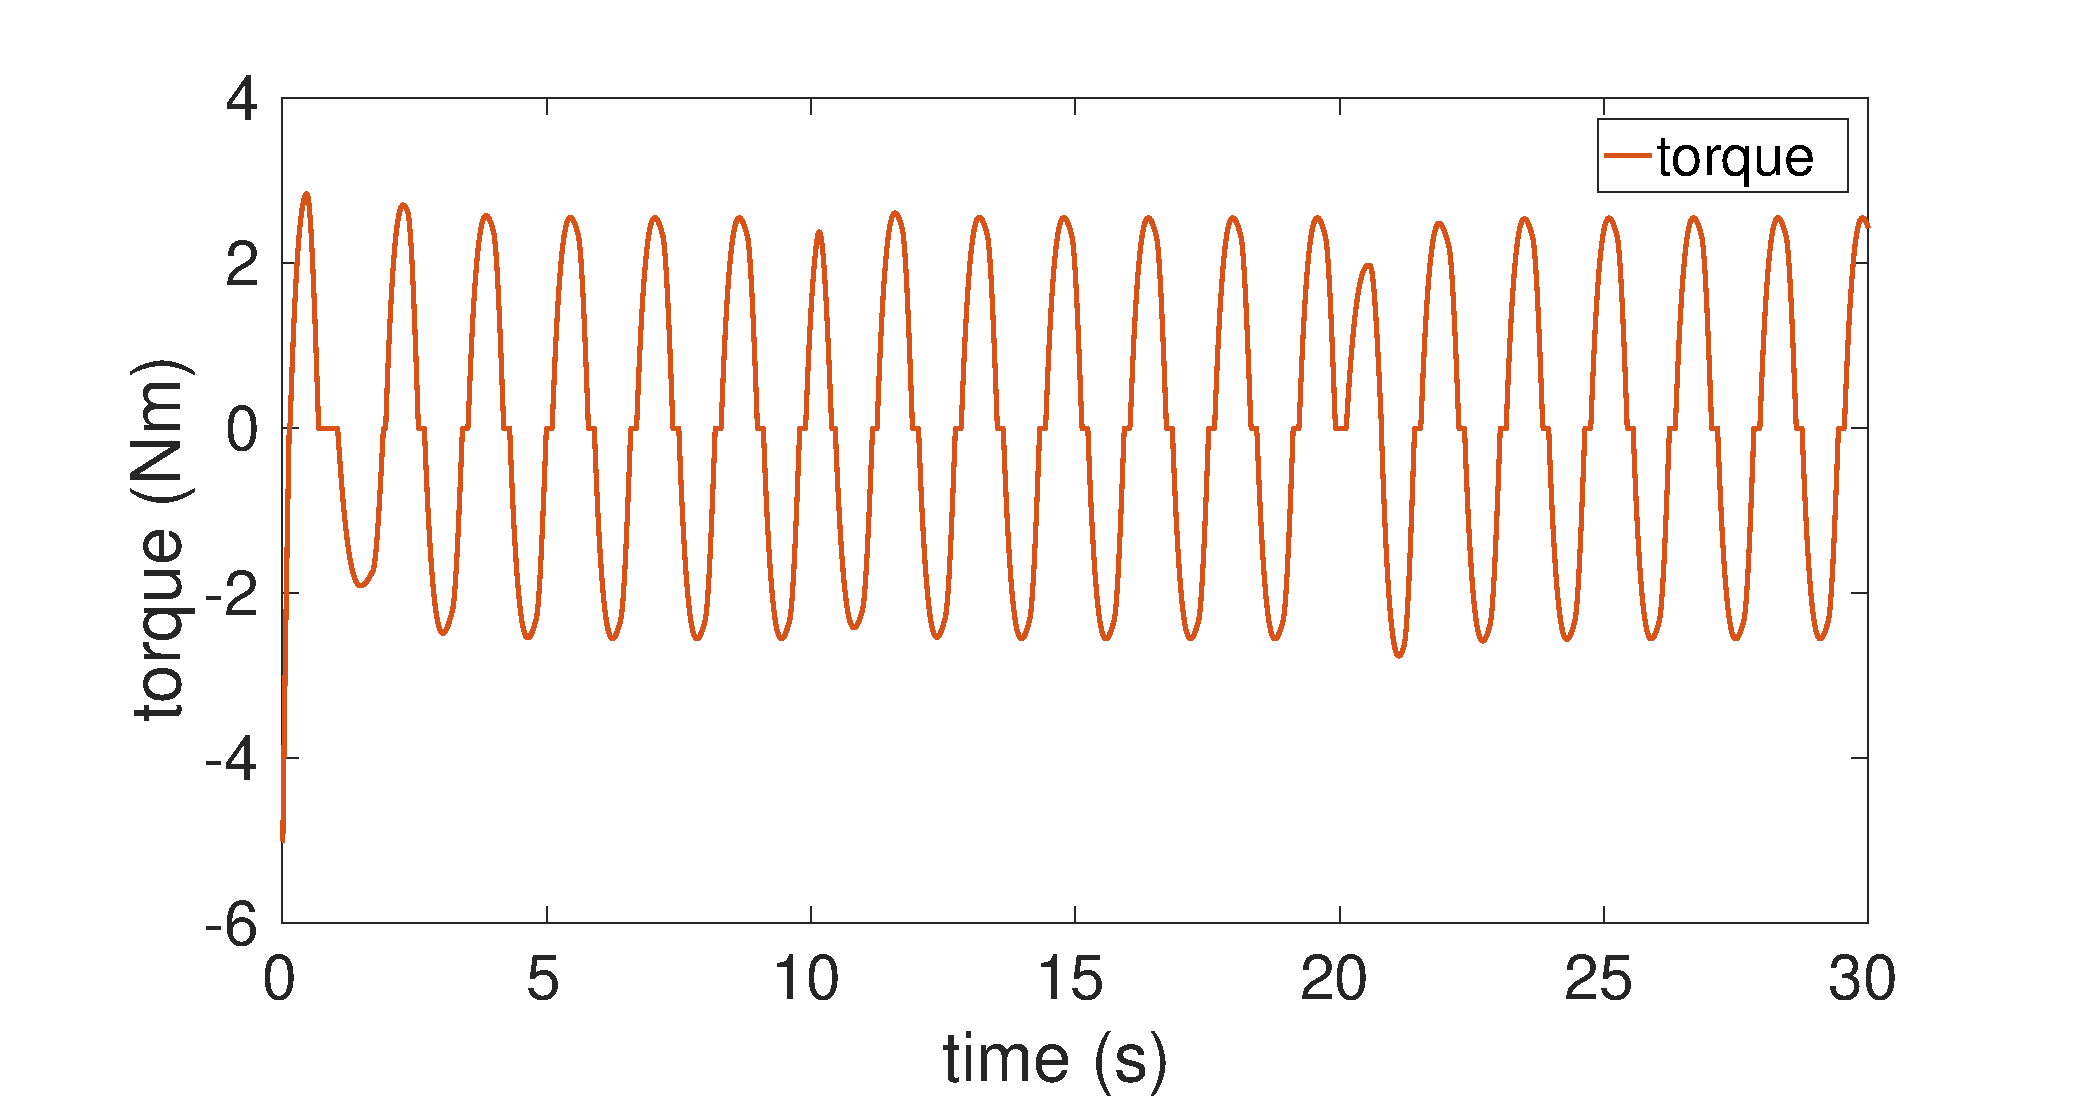
\includegraphics[scale=0.21]{figures/1-2-torque-for-change-average-position.eps}}
\subfigure[Joint position and average joint position]{\label{fig:change-avg-pos-b}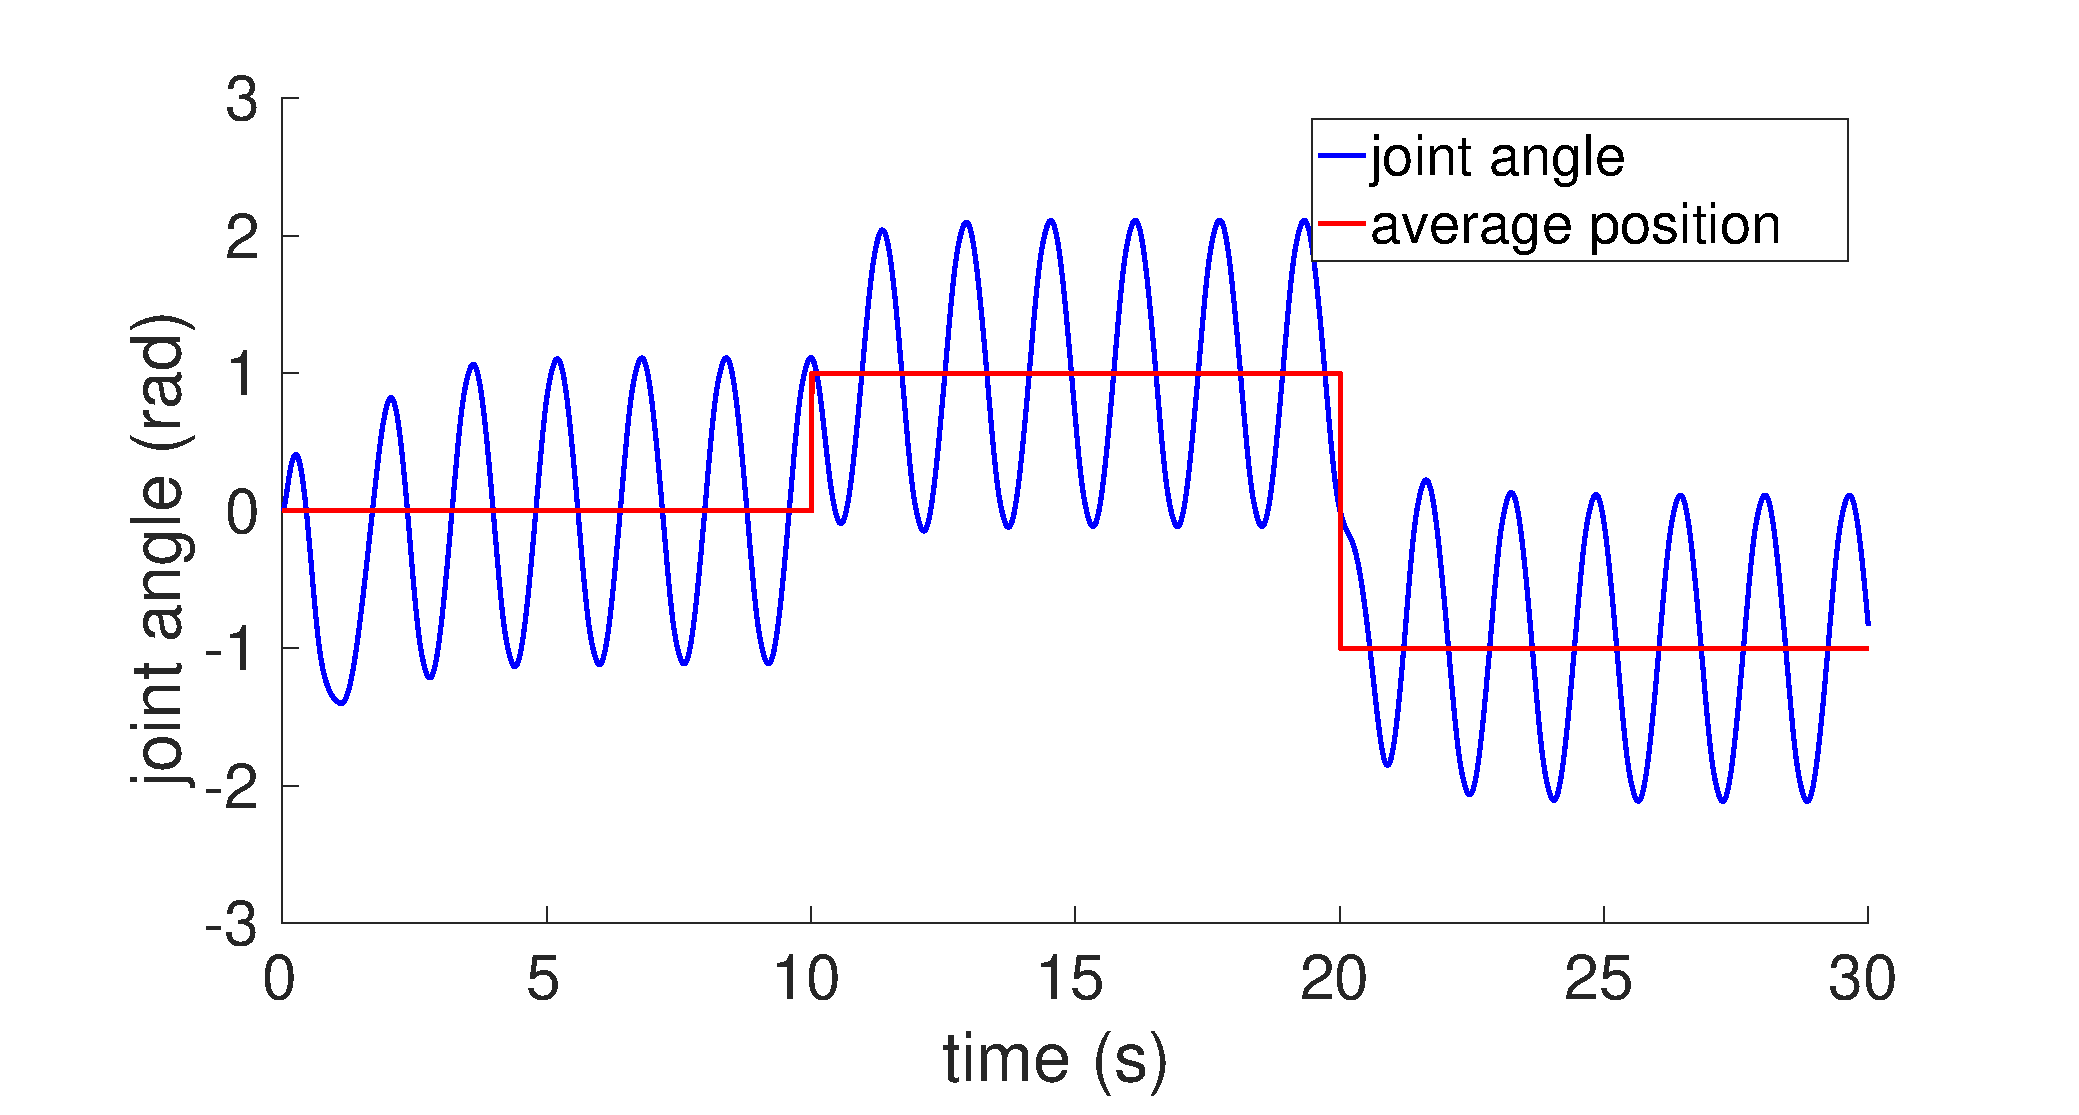
\includegraphics[scale=0.21]{figures/1-1-change-average-position.eps}}
\caption{Changing the average position of oscillation}
\label{fig:change-avg-pos}
\end{figure}

\forceindent Next, the effect of changing the tonic input is demonstrated. 
The tonic input to the oscillator is linearly related to the amplitude of the torque output and also approximately linearly to the amplitude of the position oscillations. In this example, the tonic input ($u_i,u_j$) was linearly increased from 1.0 to 4.0 over 30 seconds, and as shown in figure \ref{fig:change-amp}, the amplitude of both the oscillations increases in a linear manner. This is possible in a situation where the robot needs to change the length of its stride to move over an obstacle or to step onto a stair. As is visible from the graphs, the transitions from one amplitude to the next are smooth.

\begin{figure}[H]
\centering     %%% not \center
\subfigure[Torque output of the oscillator]{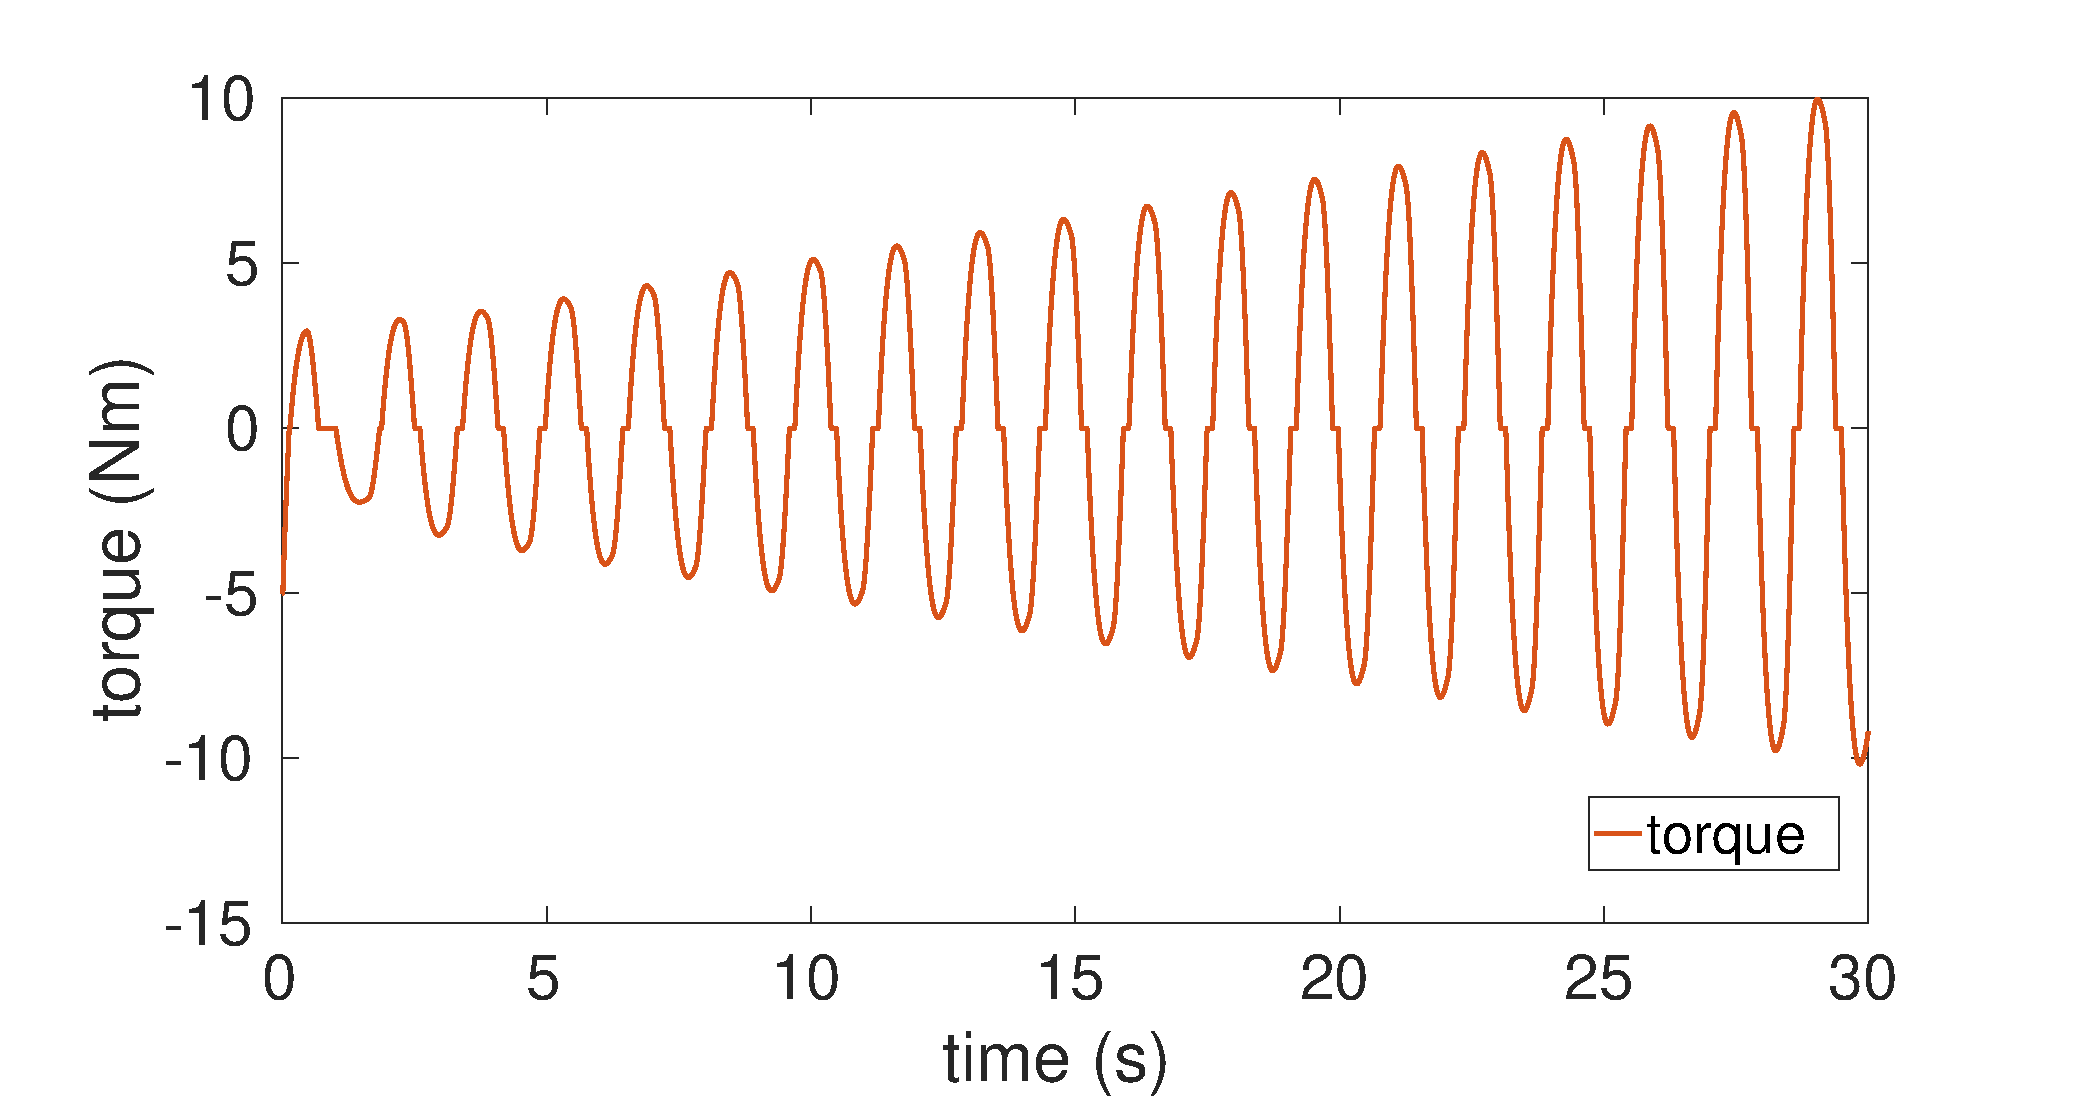
\includegraphics[scale=0.21]{figures/2-1-change-in-torque.eps}}
\subfigure[Joint position and average joint position]{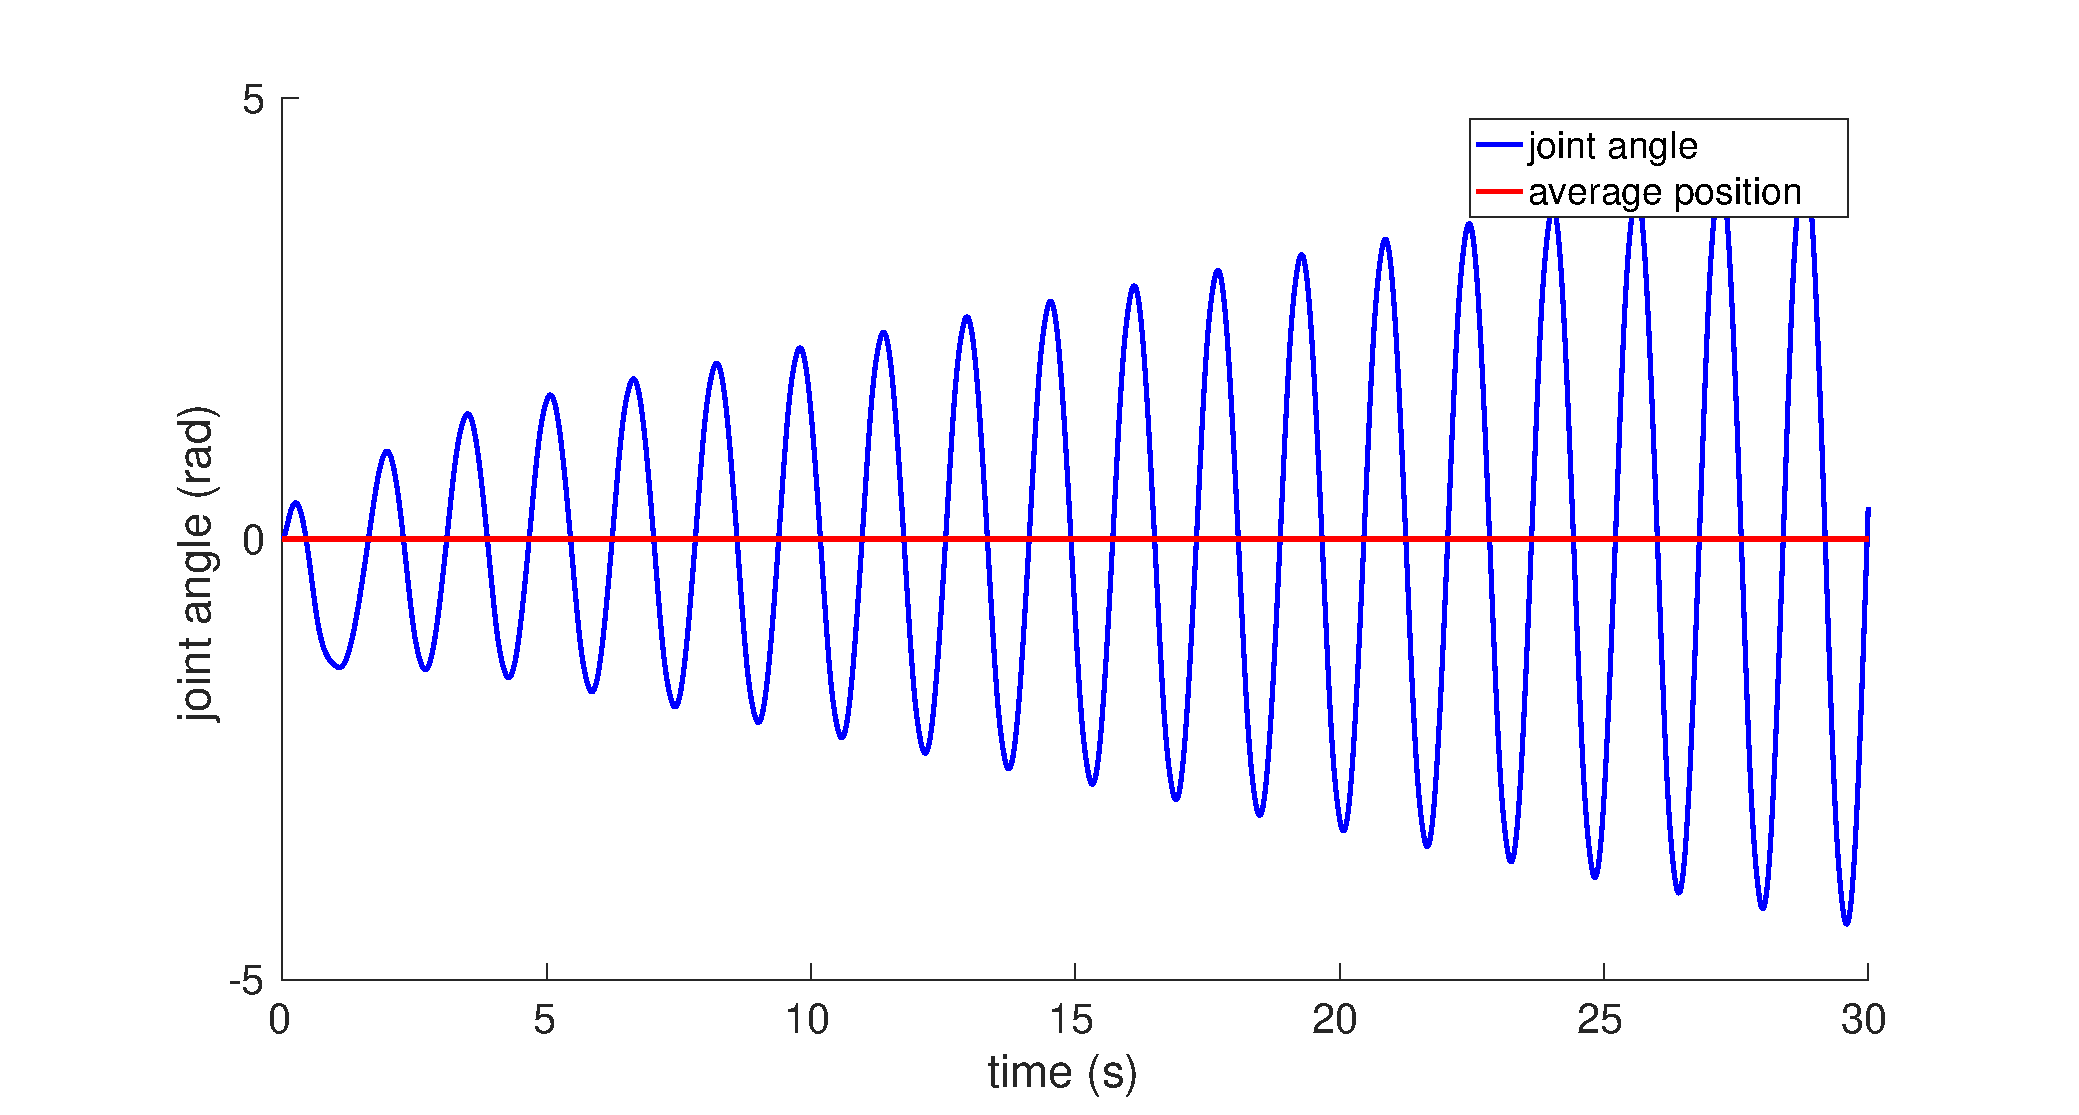
\includegraphics[scale=0.21]{figures/2-2-change-in-angle.eps}}
\caption{Changing the amplitude of oscillations}
\label{fig:change-amp}
\end{figure}

\forceindent Apart from the mean position and amplitude, another key property of a waveform is its frequency. By varying the time constant of the oscillator the frequency of the torque and joint angle oscillations can be varied. In figure \ref{fig:change-freq}, the time constant $t_1$ was set to 0.3 for the first 20 seconds, 0.6 for the next 20 seconds and to 0.9 for the last 20 seconds (only $t_1$ was modulated, the parameter $t_2$ was set as $t_2 = 2.5 \times t_1$ as in \cite{Ronsse2009}). As expected the frequency of both the torque and the joint angle oscillations decreases. However for the joint angles, the amplitude also increases as the frequency decreases. This effect maybe countered by gradually decreasing the tonic input as the frequency decreases in order to keep the amplitude constant. This kind of a situation can occur when the robot needs to change its speed of walking. Note that for both the  transitions (at $t=20s$ and $t=40s$), the changes were smooth. 

\begin{figure}[H]
\centering     %%% not \center
\subfigure[Torque output of the oscillator]{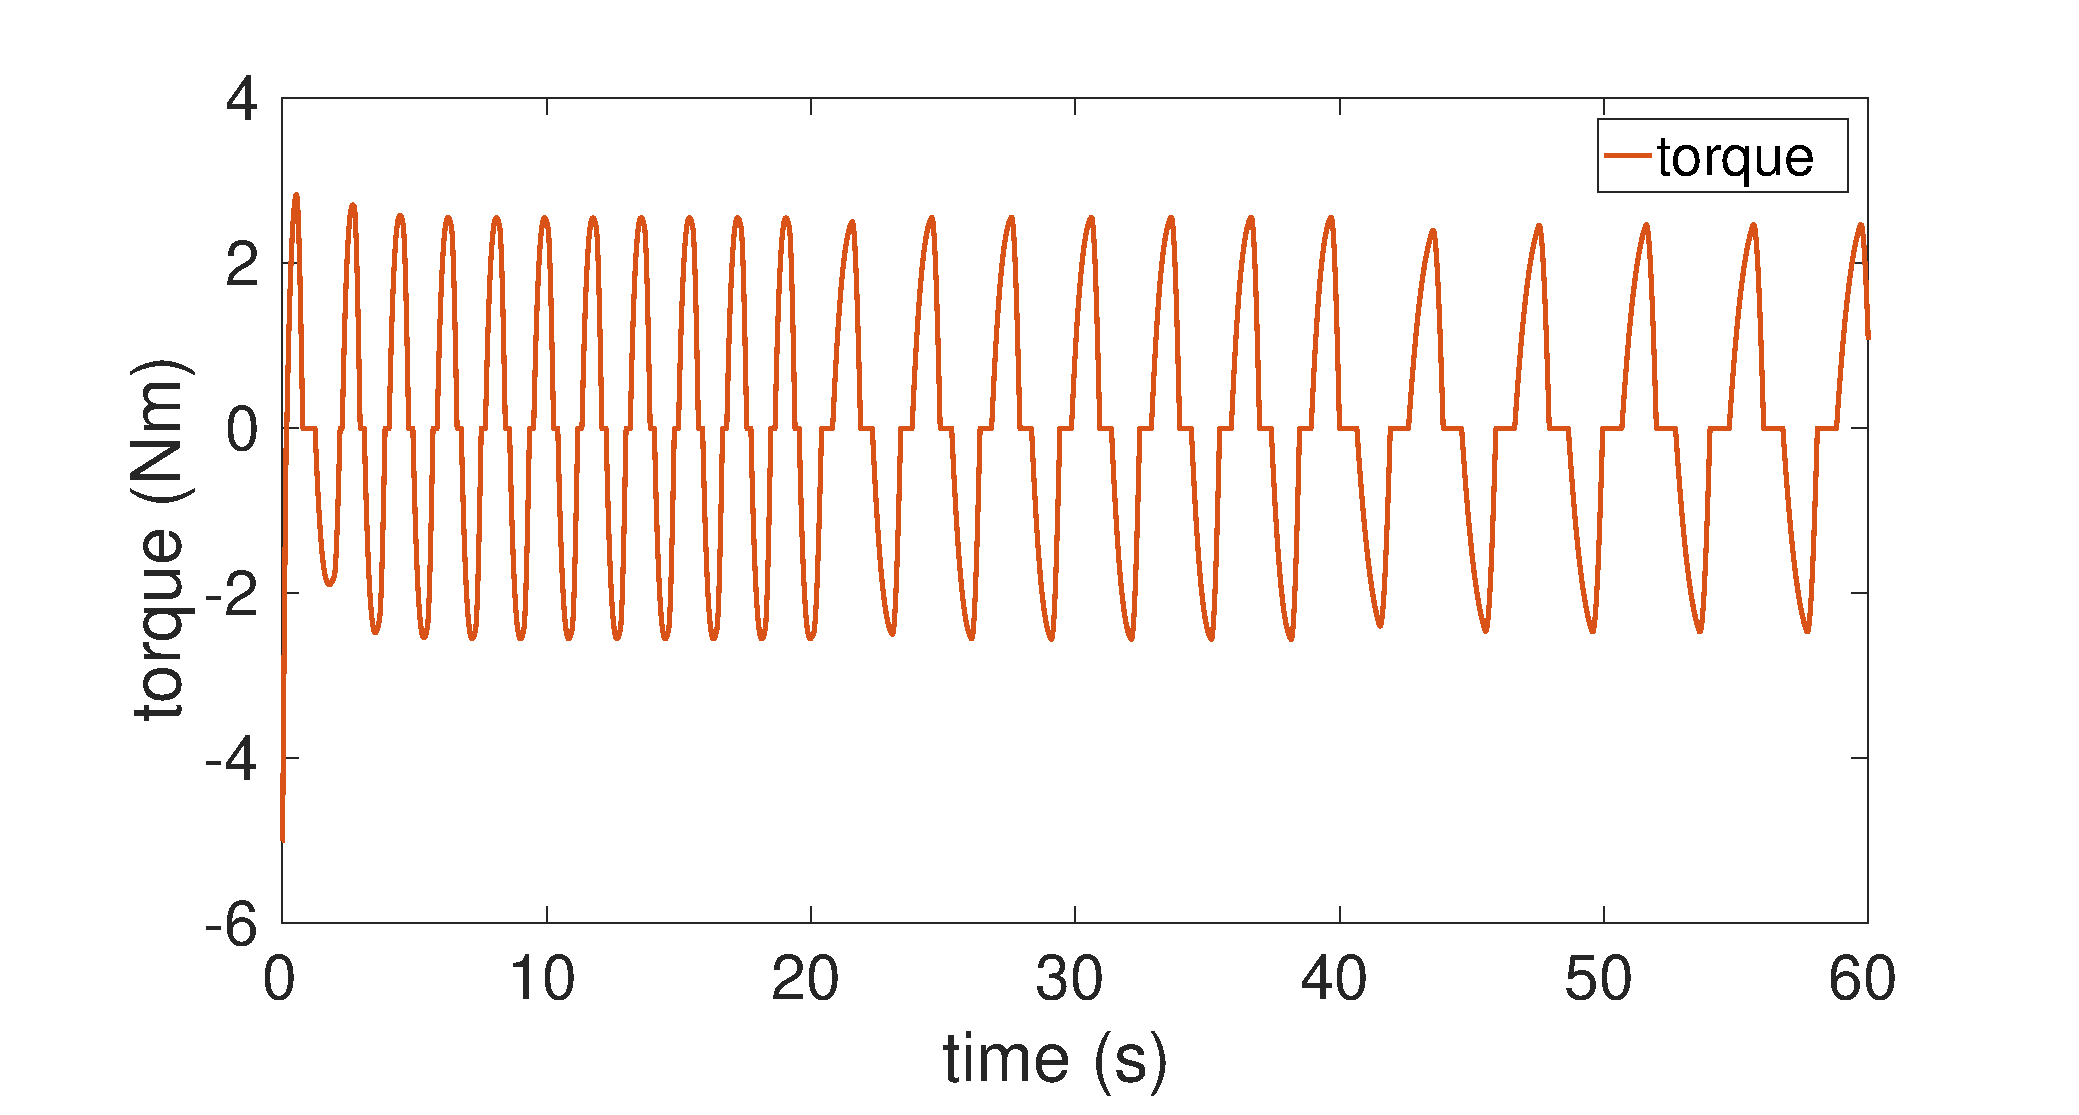
\includegraphics[scale=0.21]{figures/3-1-changing-freq-torque.eps}}
\subfigure[Joint position and average joint position]{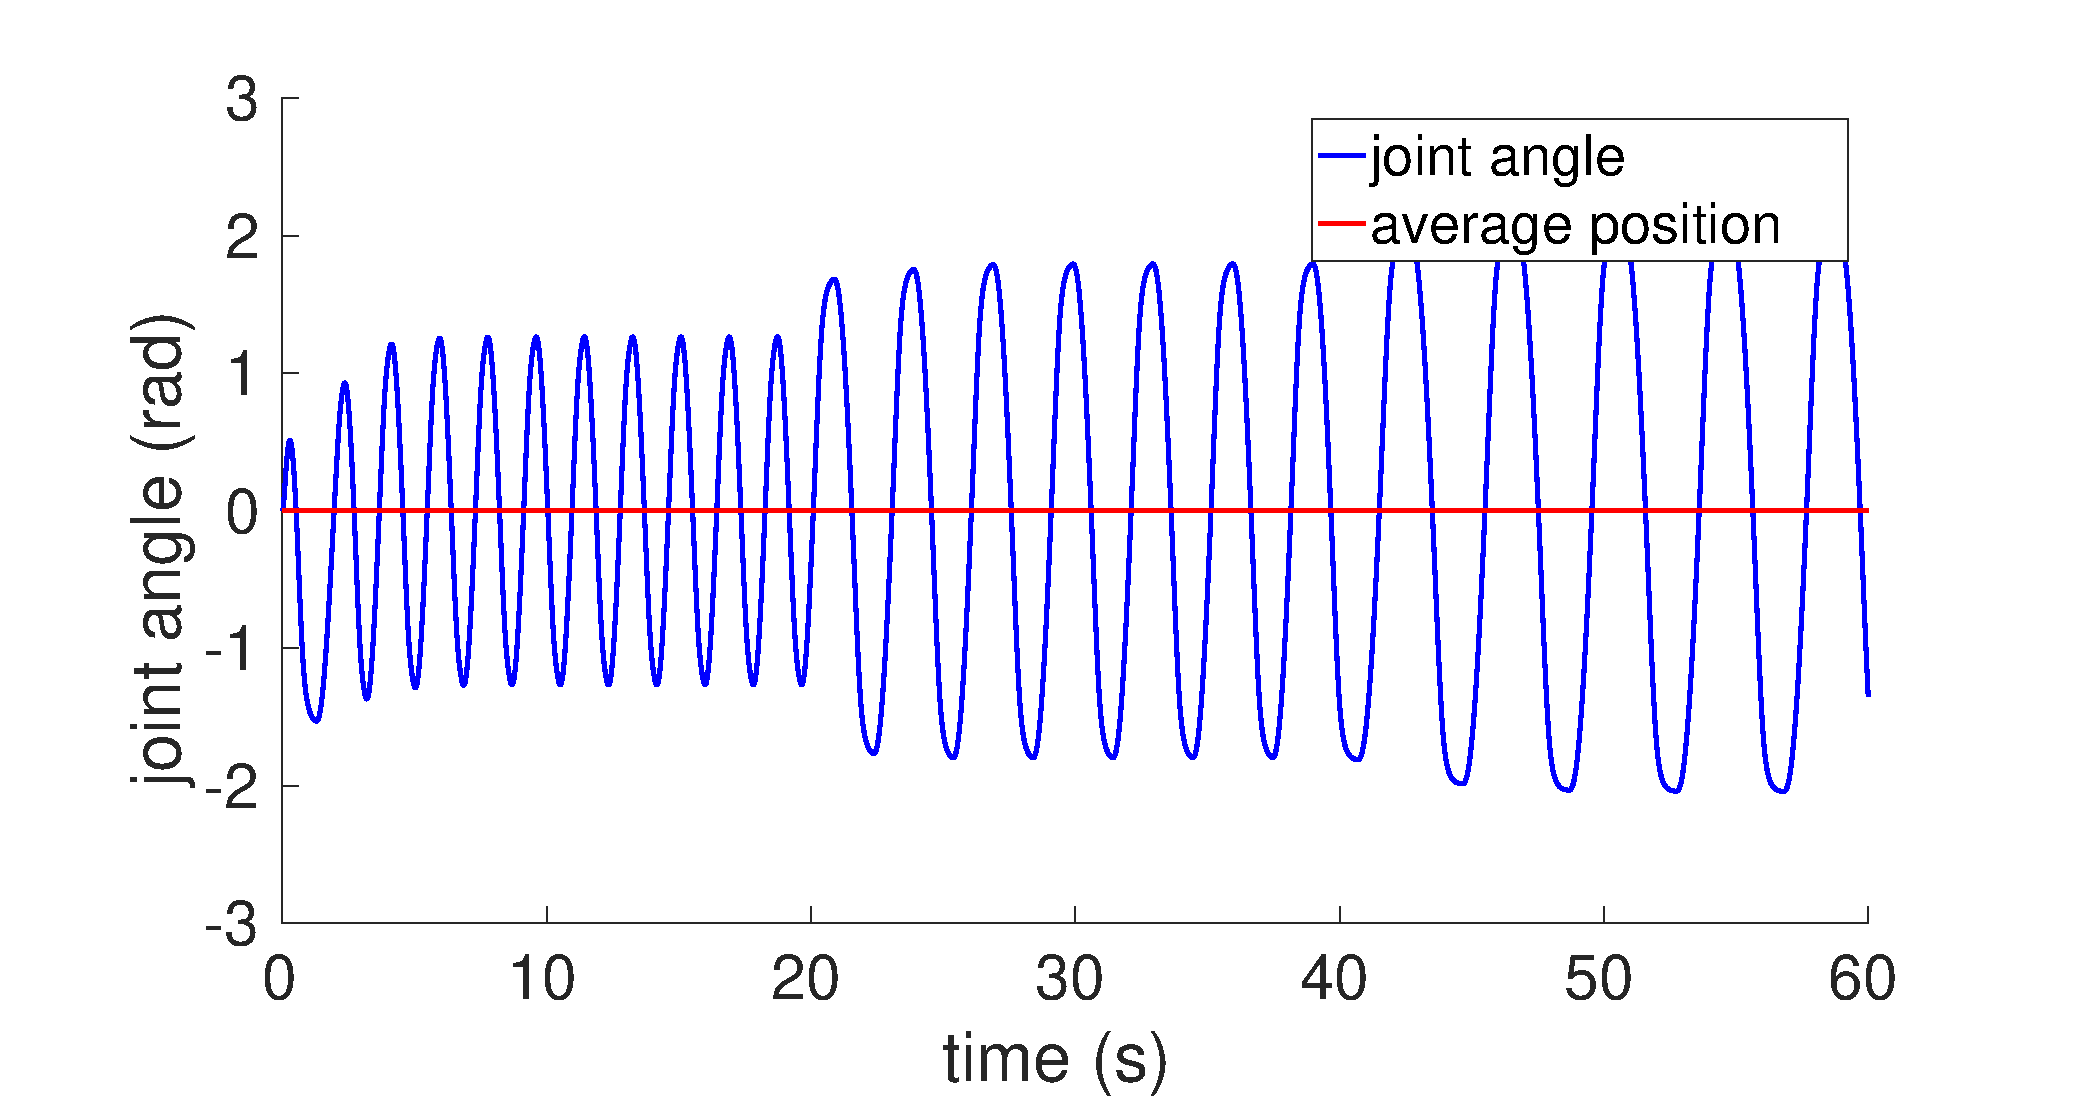
\includegraphics[scale=0.21]{figures/3-2-changing-freq-pos.eps}}
\caption{Changing the frequency of oscillation}
\label{fig:change-freq}
\end{figure}


\forceindent So far, the behavior of only a single oscillator driving a solitary joint has been described. In a robot multiple joints must interact with one another in a way that leads to a stable gait. To do so, the oscillators driving the individual joints must have a way of communicating with each other. This communication is determined by a coupling function which dictates how different oscillators can synchronize their frequencies or lock their phase \cite{Ronsse2009}. To demonstrate the effects of coupling, two oscillators driving two different joints will be considered. For convenience, the two joints may be called the left joint ($l$ subscript) and the right joint ($r$ subscript). The state variable of the left joint are $\psi_{l,i}$, $\psi_{l,j}$, $\phi_{l,i}$, $\phi_{l,j}$, $\theta_l$ and $\dot{\theta_l}$ and the tonic inputs are $u_{l,i}$ and $u_{l,j}$. Similarly the variables for the right joint are $\psi_{r,i}$, $\psi_{r,j}$, $\phi_{r,i}$, $\phi_{r,j}$, $\theta_r$ and $\dot{\theta_r}$ and the tonic inputs are $u_{r,i}$ and $u_{r,j}$. The time constants for both the joints are assumed to be $t_1$ and $t_2$. With this configuration, the coupling can be of three possible types \cite{Ronsse2009}:

\begin{enumerate}
\item \textbf{Coupled at the input level}: If $u_{r,i}=u_{l,i}$ and $u_{r,j}=u_{l,j}$, then the coupling is done at the input level. However this kind of coupling does not allow the oscillators to converge to a definite phase and they continue behaving as two independent units \cite{Ronsse2009}.
\item \textbf{Coupled at the level of internal state variables}: Here the coupling is done by having a term for $\psi_{r,i}$ in the equation of $\psi_{l,i}$ and similarly a term for $\psi_{r,j}$ in the equation of $\psi_{l,j}$ (same for the equations of the right joint). Matsuoka had suggested this kind of coupling for a network of oscillators \cite{Matsuoka1987}. The disadvantage of this type of coupling is that in a network of several oscillators, all of them will either converge to in-phase or anti-phase oscillations, and a co-existence of in- and anti-phase relation is not possible \cite{Ronsse2009}. In bipedal locomotion, the left hip joint moves in opposite phase to the right hip joint, but joints within the same leg move in-phase. Hence the coupling described here is not suitable for bipedal locomotion.
\item \textbf{Coupling at the level of output variables}: If the coupling is done at the level of the output variables $\theta_l$ and $\theta_r$, both in-phase and anti-phase relationships can be achieved within a network of oscillators \cite{Ronsse2009}. This is the coupling configuration that has been used in this paper. The equations of the oscillator, in this case become (only the equations of the right joint are given below):\\

\begin{subequations}
\label{eq:matsuoka_coupled}
%
\begin{align}
\label{eq:matsuoka_coupled1}
\begin{split}
t_1 \dot{\psi_{r,i}}={}& -\psi_{r,i} - \beta \phi_{r,i} - \eta [\psi_{r,j}]^+ - \sigma [\theta_r - \theta^{*}_r]\\ 
& - \mu [\theta_l - \theta_l^*]^+ - \nu [-\theta_l + \theta_l^*]^+ + u_{r,i} 
\end{split}
\\
%
\label{eq:matsuoka_coupled2}
t_2 \dot{\phi_{r,i}} = {}& -\phi_{r,i} + [\psi_{r,i}]^+
\\
%
\label{eq:matsuoka_coupled3}
\begin{split}
t_1 \dot{\psi_{r,j}}={}& -\psi_{r,j} - \beta \phi_{r,j} - \eta [\psi_{r,i}]^+ - \sigma [\theta_r - \theta^{*}_r]\\
& - \mu [\theta_l - \theta_l^*]^+ - \nu [-\theta_l + \theta_l^*]^+ + u_{r,j}
\end{split}
\\
%
\label{eq:matsuoka_coupled4}
t_2 \dot{\phi_{r,j}} ={}& -\phi_{r,j} + [\psi_{r,j}]^+
\end{align}
%
\end{subequations}

In this setup equations \ref{eq:matsuoka_net_torque} and  \ref{eq:inertial_system} remain unchanged. $\mu$ represents the constant for homologous coupling (since it is similar to the effect induced by $\sigma$ but for the other joint) and $\nu$ is the constant for non-homologous coupling. All other symbols have the same meaning as in equations  \ref{eq:matsuoka_basic}-\ref{eq:matsuoka_phi} \cite{Ronsse2009}.
\end{enumerate}

\begin{figure}[htbp]
\centering     %%% not \center
\subfigure[Anti-phase oscillations]{\label{fig:anti-phase}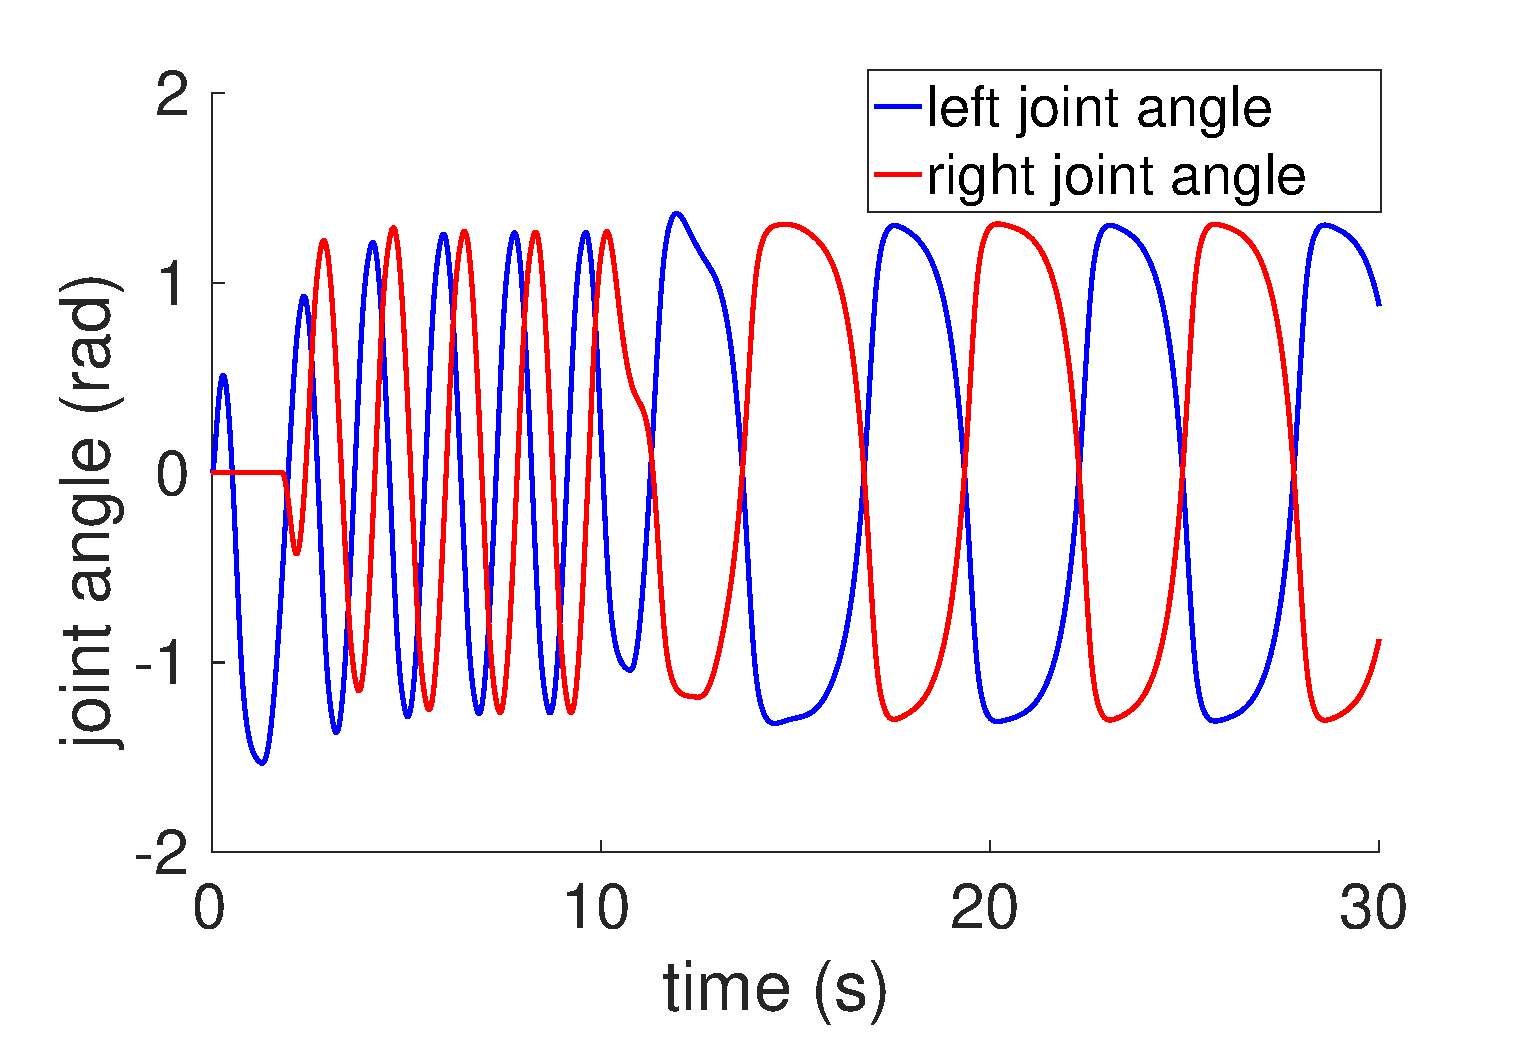
\includegraphics[scale=0.28]{figures/4-1-anti-phase.eps}}
\subfigure[In-phase oscillations]{\label{fig:in-phase}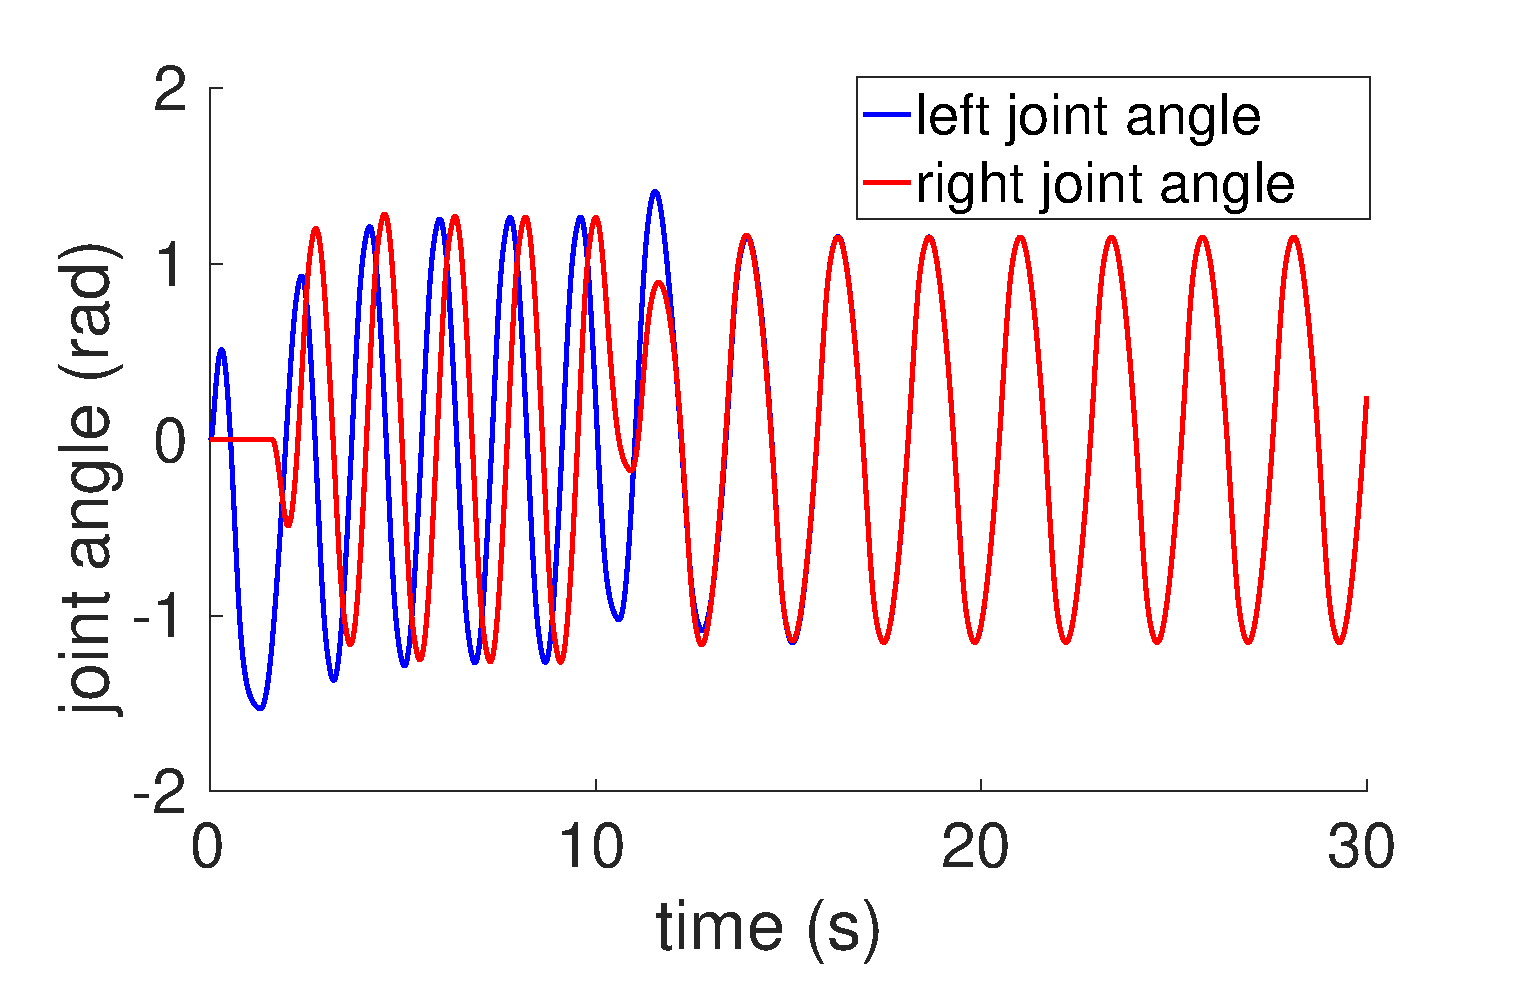
\includegraphics[scale=0.28]{figures/4-2-in-phase.eps}}
\caption{Anti-phase and in-phase oscillations}
\label{fig:in-anti-phase}
\end{figure}

\forceindent By using equations \ref{eq:matsuoka_coupled}, \ref{eq:matsuoka_net_torque} and  \ref{eq:inertial_system}, the behavior of a system of coupled oscillators can be demonstrated, as depicted in figure \ref{fig:in-anti-phase}. The values of the constants used are $t_1=0.3$, $t_2= 2.5 \times t_1$ as per \cite{Ronsse2009} (same for left and right joints), $\beta=2.5$,  $\eta=2.5$, $\sigma=1.5$, $\theta^*=0.0$, $h_{\psi}=5.0$, $\mu=0.75$, $\nu=0.49$ and $u_{l,i}=u_{l,j}=u_{r,i}=u_{r,j}=1.0$. These values were selected based on \cite{Ronsse2009}. For both the types of oscillations, the oscillator of the right joint is started a little while after the oscillator of the left joint, in order to introduce an initial phase difference. For 10 seconds, the two oscillators behave independently of each other and do not settle into any fixed phase-relationship. However as soon as the coupling is turned on at t=10s, the two oscillators converge to either anti-phase or in-phase oscillations. For anti-phase oscillations, the right oscillator is started 1.68s after the left oscillator and for the in-phase oscillation, it is started after 1.67s. Thus it is evident that the initial phase difference between the oscillators also plays a part in determining which kind of phase-relationship the oscillators converge to.\\
\forceindent Another important characteristic of this system of coupled oscillators is that the final phase difference between the two oscillators can either be 0 (in-phase) or $\pi$ radians (anti-phase). No other phase-relationship is possible. In order to demonstrate this characteristic, the system of two oscillators was tested out with a range of different initial phase differences (using difference of activation times) and time periods of oscillation. An empirical formula ($T=1.47t_1 + 2.92\sqrt{t_1} - 0.2304$) for calculating the joint oscillation time period in terms of the time constant $t_1$ was used \cite{Ronsse2009}. The final phase difference between the two waveforms was calculated by using the Hilbert Transform. Figure \ref{fig:stable-attractors} confirms that for any initial phase difference and any time period of oscillation, the oscillators converge to either in-phase or anti-phase oscillations. It can also be seen that the basin of attraction of in-phase oscillations is larger than that of anti-phase oscillations.

\begin{figure}[htbp]
\centering
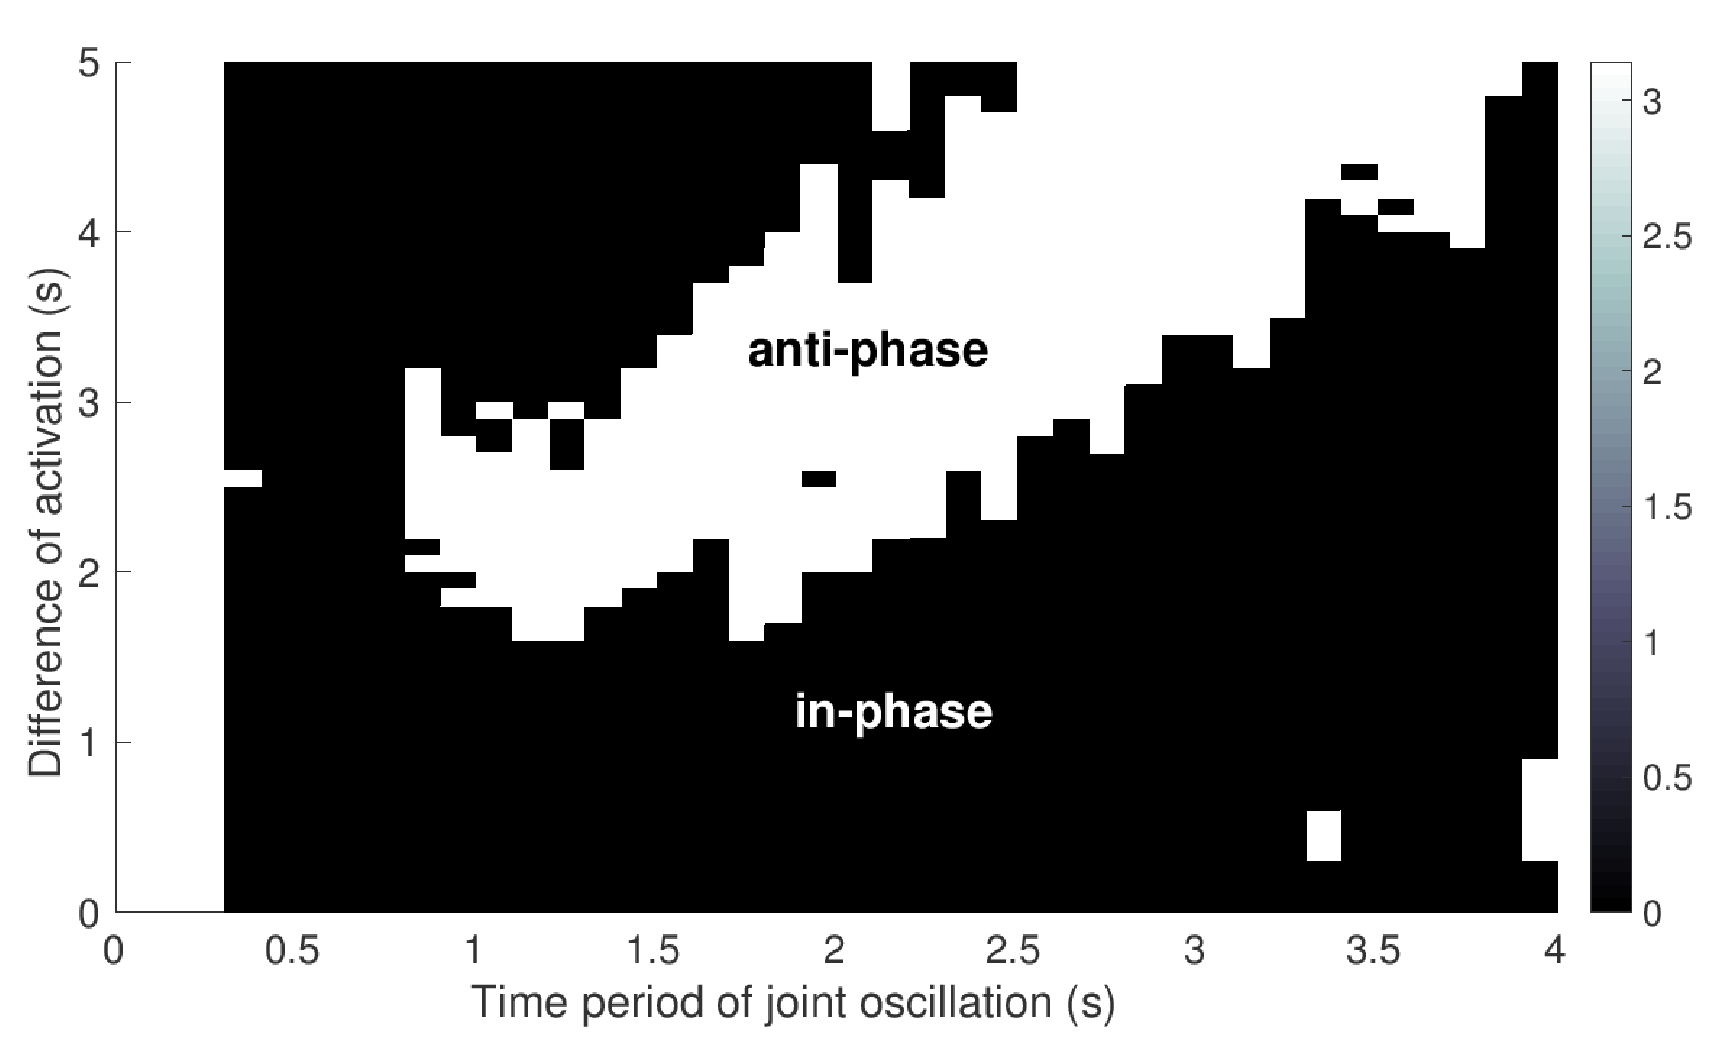
\includegraphics[scale=0.3]{figures/5-1-stable-attractors.eps}
\caption{The joint oscillations converge to only 2 modes - either in-phase or anti-phase (based on \cite{Ronsse2009}).}
\label{fig:stable-attractors}
\end{figure}

\section{Robot Joint Control}
\label{sec:Robot_Joint_Control}
The concept of using CPGs in bipedal robots is not new. Several studies in the past have tried to utilize CPGs, particularly the Matsuoka oscillator, to develop walking algorithms. However, most of these studies such as \cite{Taga1991}, \cite{nakanishi2004learning}, \cite{Ishiguro2003} have used custom built torque driven robot models. Although these papers present useful insights into bipedal walking, it is very difficult to implement the methods on commercially available robots, almost all of which are position controlled (robot control is in terms of the joint angles and not in terms of joint torque). Some studies which do use commercial robots like the Nao, such as \cite{cristiano2014locomotion}, have used Matsuoka oscillators in master-slave configurations to drive robot joints. In this case, utilizing the properties of the oscillator (as discussed in section \ref{sec:Matsuoka_Oscillator}) becomes very difficult. Therefore, in this paper, an effort has been made to use the Matsuoka oscillator in a novel configuration which can be implemented on a commercially available position controlled robot, and also utilizes the oscillator's properties.\\
\forceindent If the equations of the system of coupled Matsuoka oscillators are investigated (equations \ref{eq:matsuoka_coupled} and \ref{eq:matsuoka_net_torque}), it can be seen that the output $\psi_T$ of the oscillators is the torque that should be exerted at the joints, while the feedback is only in terms of the joint angle at a given time $\theta_l$ or $\theta_r$. In a torque based control system, the system generates target torques and uses the feedback in the form of actual torques to make the necessary corrections, but for the Matsuoka oscillator (as used here), this is not the case. This is an important property which can be exploited to use the Matsuoka oscillator in a position controlled robot.

\begin{figure}[htbp]
\centering
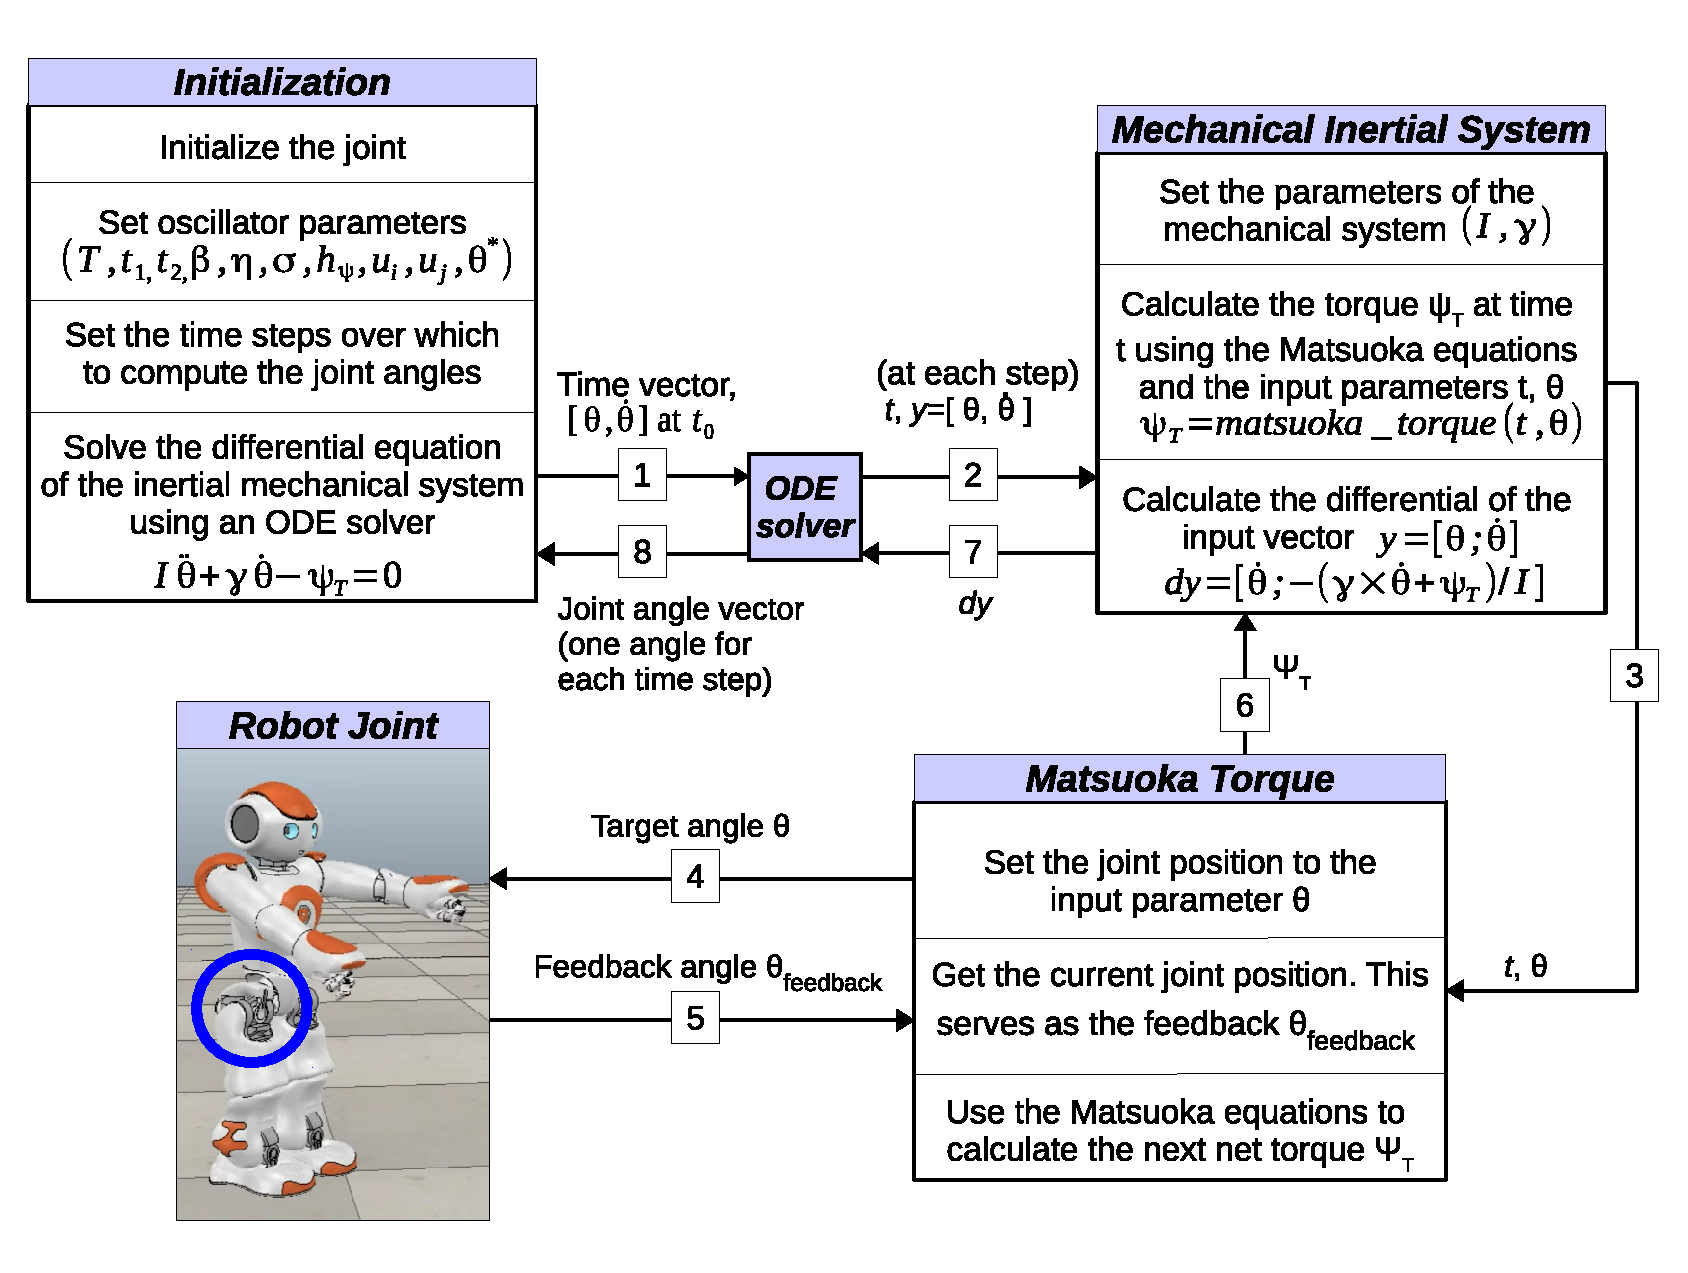
\includegraphics[scale=0.5]{figures/robot_joint_control.eps}
\caption{Using the Matsuoka oscillator in a position controlled robot}
\label{fig:robot_joint_control}
\end{figure}

\vspace{10pt}

\textbf{Matsuoka oscillator driving a position controlled joint}: As shown in figure \ref{fig:robot_joint_control}, first the joint is initialized to 0 radians and then the oscillator parameters are set. The empirical formula for the oscillation time period ($T=1.47t_1 + 2.92\sqrt{t_1} - 0.2304$ \cite{Ronsse2009}) is used to derive the parameters $t_1$ and $t_2$; $t_1$ is calculated as $t_1=2.13 + 0.6804T - \sqrt{4.512 + 2.685T}$ and $t_2$ is calculated as $t_2=2.5 \times t_1$ (derivations are as per \cite{Ronsse2009}). The other parameters are set to suitable values, and the time vector is also set (total duration and duration of each time step). After this an Ordinary Differential Equation (ODE) solver is used to solve the differential equation of the mechanical inertial system (equation \ref{eq:inertial_system}). At each time step, the ODE solver calls a module which computes the derivative of $[\theta, \dot{\theta}]$ (vector made up of the angular position and velocity). To compute the derivative, the module of the mechanical inertial system calculates the net torque first. It passes the target angle to the Matsuoka torque module, which in turn sends it to the robot to be executed on the appropriate joint. The robot senses the actual angle of the joint ($\theta_{feedback}$) and the torque for the next step is computed using the sensed angle. This torque $\psi_T$ is returned to the mechanical inertial system module, and finally the derivative of $[\theta, \dot{\theta}]$ is calculated and sent back to the ODE solver. The same process is repeated for each time step till the previously fixed final time is over.\\

\forceindent The important thing to note about the process described above is that the computed torque $\psi_T$ is not applied to the joint at all. It is treated like an intermediate variable that is only required to calculate the target joint angle $\theta$. Use of the feedback angle $\theta_{feedback}$ ensures that the joint moves as desired. Hence the parameters of the inertial system ($I$ and $\gamma$) can be set to any value (as long as they do not cause oscillations to disappear) and do not need to accurately model the physical joint properties. It is also worth mentioning that in this implementation, normally available ODE solvers such as the Runge-Kutta solvers cannot be used. The reason is that these solvers use variable time steps to optimize the process and sometimes traverse back in time to minimize the approximation error. In the current scenario, the ODE solver has to internally use the Matsuoka equations which depend on state variables with persistent values. Going back in time can corrupt these state variables leading to incorrect results. Hence, a custom ODE solver which uses fixed time steps, was used here.\\
\forceindent Using the process described in figure \ref{fig:robot_joint_control}, multiple joints can also be controlled (with the help of equation \ref{eq:matsuoka_coupled}). For testing this process, Matsuoka oscillators were used to control the shoulder joints of a Nao robot in simulation. The two shoulder joints were driven first in anti-phase and then in-phase, and the graphs similar to that of figure \ref{fig:in-anti-phase} were reproduced by using the robot. Apart from this, another kind of movement is important in bipedal robots. It is the movement of coupled joints which start in-phase and then one joint moves with a frequency that is a multiple of the other joint's frequency. This relationship exists between the joints of the knees and the hip, with the knees moving at twice the frequency of the hip. In order to show this effect on a stationary robot, one shoulder joint was moved at approximately twice the frequency of the other (figure \ref{fig:nao_joint_motion}). In this case, some parameters were  different for the two oscillators (indicated by the use of an additional subscript - $l$ for left and $r$ for right). The parameters used were $T_l=2.4$ ($t_{l,1},t_{l,2}$ are calculated as described above), $u_{l,i}=u_{l,j}=0.5$, $T_r=1.2$ ($t_{r,1},t_{r,2}$ are calculated as described above), $u_{r,i}=u_{r,j}=1.0$, $\beta=2.5$, $\eta=2.5$, $\sigma=1.5$, $\mu_l=0.375$, $\mu_r=0.75$, $\nu_l=0.245$, $\nu_r=0.49$, $h_\psi=5.0$. All these values were arrived at empirically. The resulting motion is depicted in video number 7 in \cite{Vid_Nao_Matsuoka}. The other motions generated in the Nao can also be viewed in \cite{Vid_Nao_Matsuoka}.

\begin{figure}[H]
\centering     %%% not \center
\subfigure[Snapshots from video\# 7 in \cite{Vid_Nao_Matsuoka}, joints moving with different frequencies]{\label{fig:nao_motion}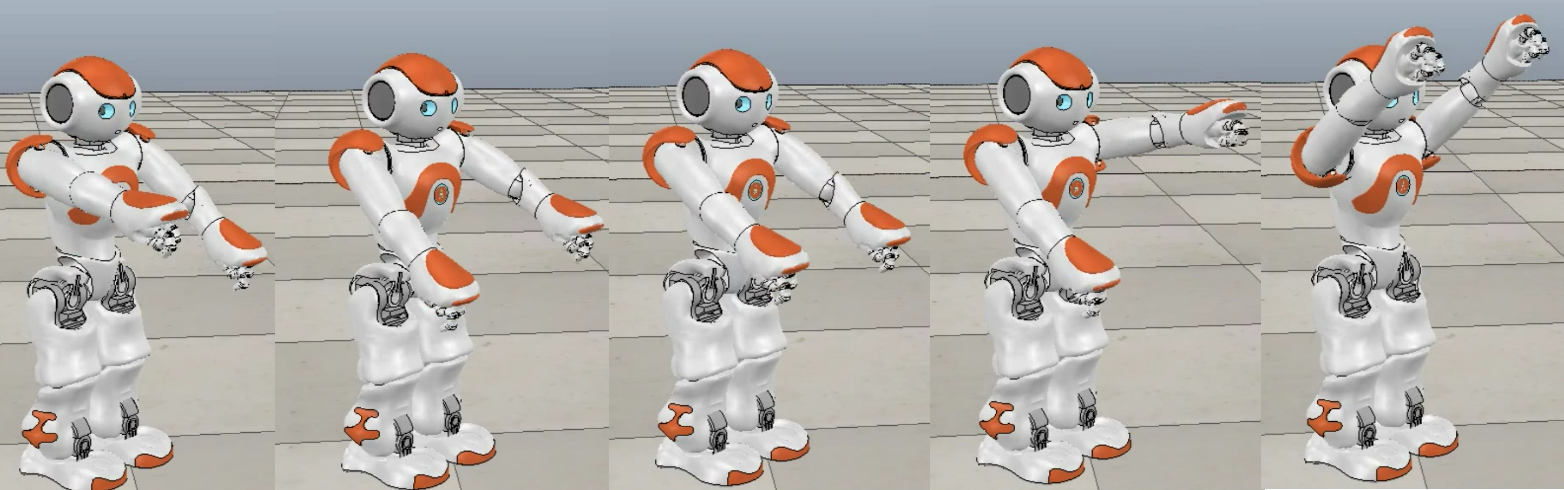
\includegraphics[scale=0.12]{figures/nao_joint_motion.png}}
\subfigure[Two joints moving in-phase but with different frequencies. Coupling is switched on at t=10s]{\label{fig:nao_graph}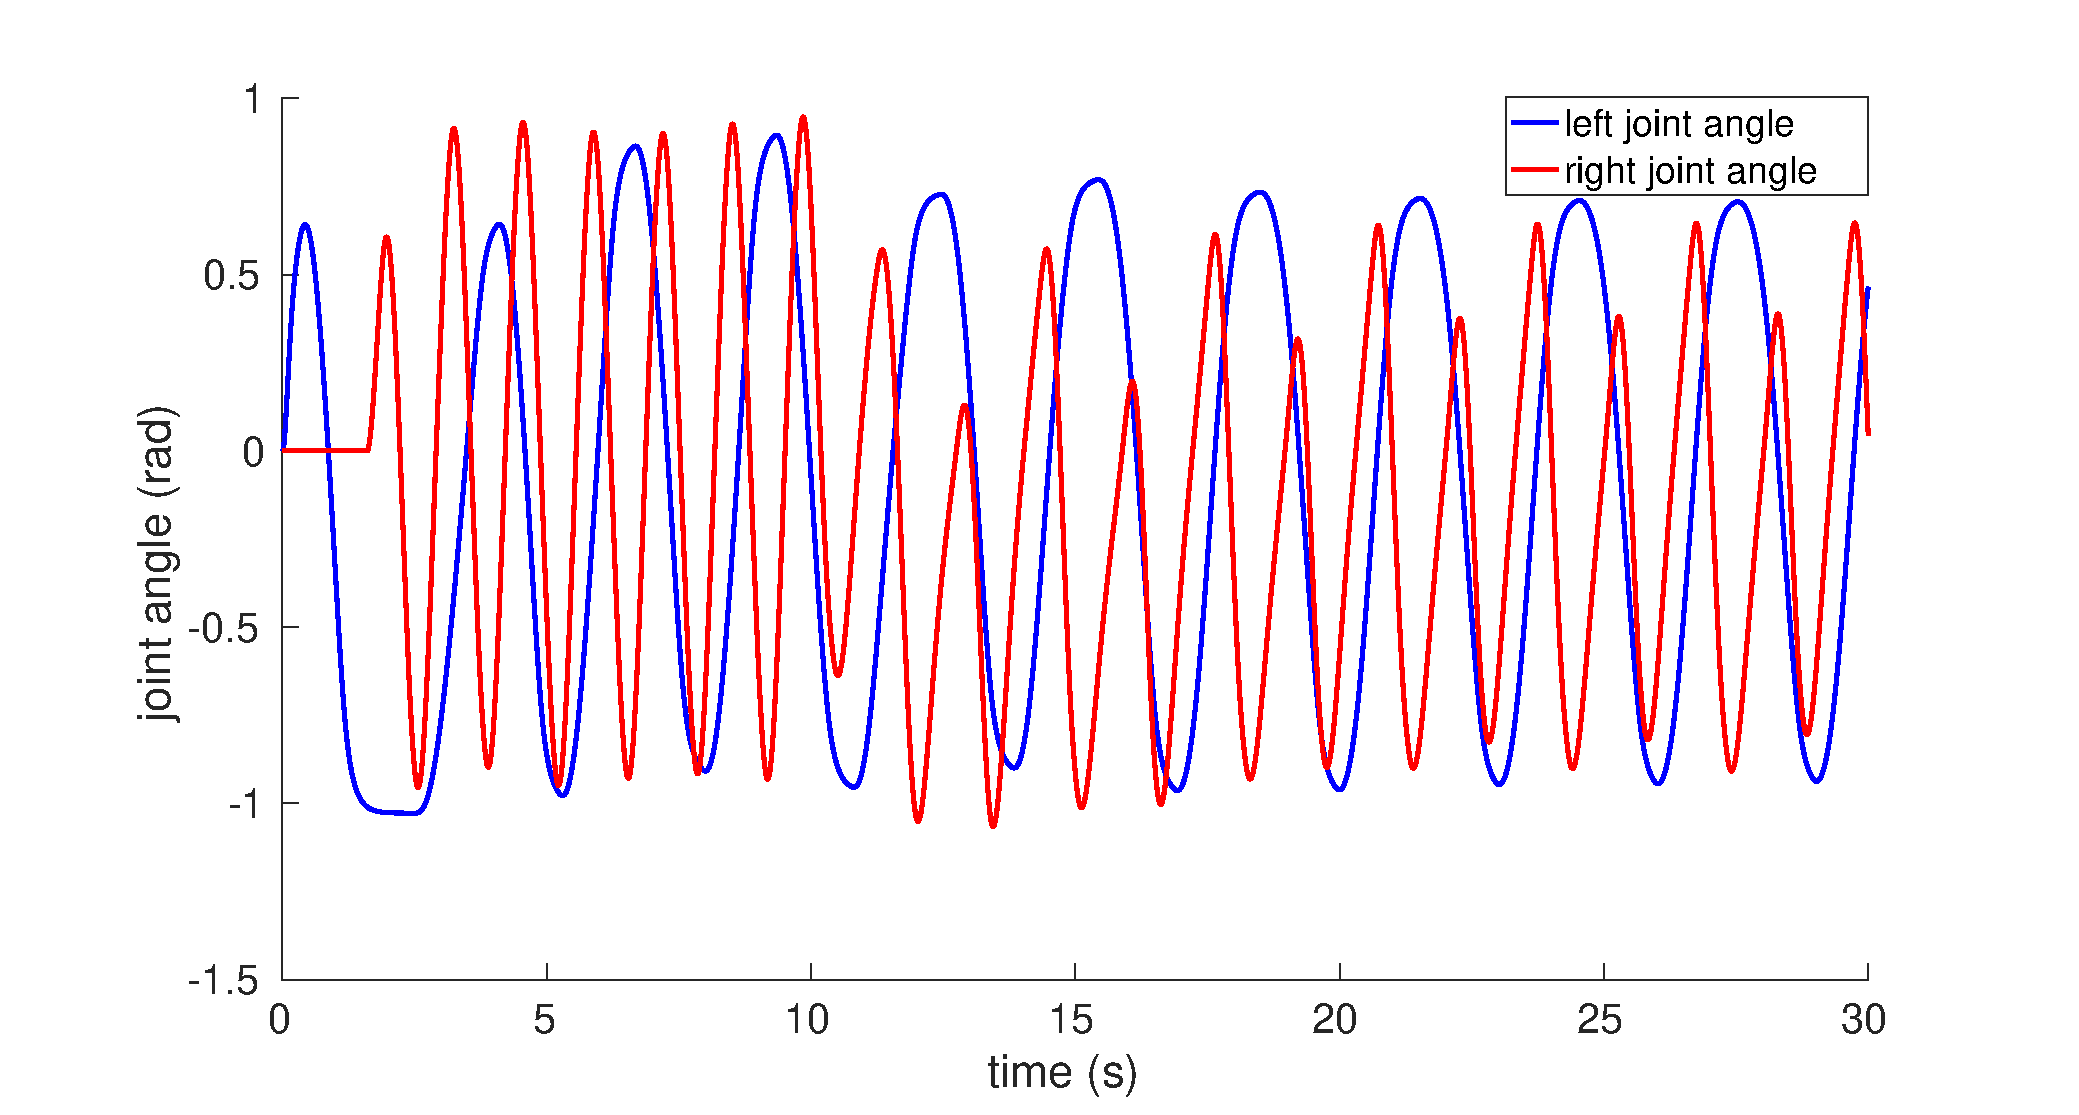
\includegraphics[scale=0.24]{figures/double-joint-in-phase-diff-freq.eps}}
\caption{Coupled joint oscillations in the robot}
\label{fig:nao_joint_motion}
\end{figure}


\section{Future Work}
\label{sec:Future_Work}
In section \ref{sec:Robot_Joint_Control} it was demonstrated that it is possible to control a position controlled robot using the Matsuoka oscillator. Using a similar setup a network of oscillators can be used to control the individual joints in a way that leads to a stable gait. Future work in this regard will involve determining the set of parameters that when implemented on the network of oscillators produces synchronized joint oscillations and helps the robot to walk on a flat even surface.\\
\forceindent A possible way of connecting several oscillators so as to form a network is shown in figure \ref{fig:future_work} (bottom-right). Here each oscillator consists of 2 half center neurons as depicted in figure \ref{fig:half_center}. An oscillator may be coupled to one or more oscillators by means of the coupling constants $\mu$ and $\nu$ as used in equation \ref{eq:matsuoka_coupled}. Each oscillator contains a large number of parameters and hence for a network of $10$ oscillators together with the associated couplings, the number of parameters is quite large. In order to reduce the parameter space, the symmetry inherent in bipedal locomotion can be utilized. Hence the parameters for an oscillator of the left leg can be made equal to the parameters of the corresponding oscillator from the other leg ($L1$ with $R1$ and so on). For the couplings too, a similar approach can be followed.

\begin{figure}[hbtp]
\centering
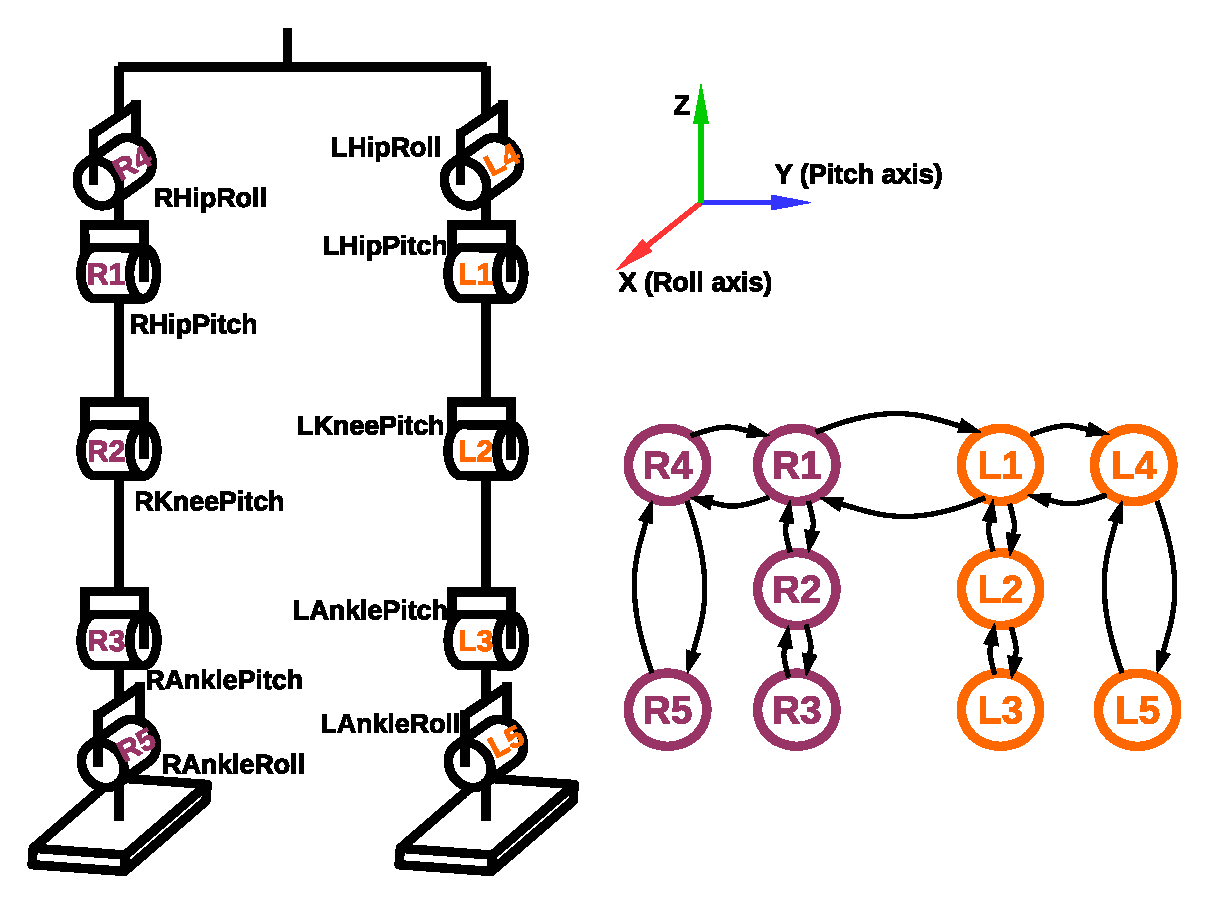
\includegraphics[scale=0.5]{figures/future_work_oscillator_network.eps}
\caption{(left) The joints in the legs of the Nao robot which are used for walking. Labels beside the joints denote the joint names and the coloured labels on the joints denote the oscillator which controls the joint. (top-right) Joint rotation axes. (bottom-right) The oscillator network which will  control the joints. Arrows denote the coupling between different oscillators.}
\label{fig:future_work}
\end{figure}

\forceindent Once a suitable parameter set has been identified, optimization algorithms can be used to find parameter values that result in a stable walk. For this, the oscillator network will be initialized with different parameter values and the robot will be tested in simulation in an attempt to find the ideal set of parameter values. For the optimization, Particle Swarm Optimization \cite{Eberhart1995, Shi1998, Kennedy2002} and a few of its variants such as the ATRE-PSO (a type of diversity guided Attraction-Repulsion PSO) \cite{Pant2007a} and QI-PSO (Quadratic Interpolation PSO) \cite{Pant2007} can be used. Since the number of parameters is quite high, ATRE-PSO and QI-PSO are suitable choices, as they have been shown to perform well on high dimensional problems.\\
\forceindent If the PSO algorithms are successful in discovering a stable gait, then the next step will be to implement a balance controller that will utilize real time information from the robot's sensors (both proprioceptive sensors and other integrated sensors such as the gyroscope or accelerometer) to make minor modifications to the robot's gait so that it can stabilize itself when dealing with an uneven surface or with random forces. The modifications will be in the form of minor adjustment to the oscillator parameters that have been optimized by the PSO algorithms. A synergy between the oscillator network, balance controller and the robot hardware will hopefully result in a system that is able to tackle both even terrain and moderately uneven terrain. 

\section{Conclusion}
\label{sec:Conclusion}
Central Pattern Generators such as the Matsuoka oscillator are potentially an excellent alternative to the widely accepted ZMP based techniques of bipedal walking. CPGs are beneficial in many ways, the most important being their ability of exploiting the natural dynamics of the mechanical structure instead of suppressing it. Using a hierarchical walking controller, where the CPGs are responsible for pattern generation and form the lowest level, has the added advantage of making things very simple for the higher level balance controller. The balance controller only needs to convey control signals for overall posture and walking direction and does not need to bother with low level joint trajectories.\\
\forceindent Although the Matsuoka oscillator has been around for a few decades, its use was somewhat restricted by the fact that most commercially available robots are position controlled and the Matsuoka oscillator generates torques which cannot be directly used in such robots. With the development of the technique discussed in this paper this limitation can be overcome. What is also interesting in this respect is that a CPG based framework for walking can be easily adapted to any biped robot and is not tightly coupled with a particular hardware setup. Thus very little additional effort will be required to create a similar setup for different robots.\\
\forceindent Biologically inspired techniques have been used to solve many intractable problems in artificial intelligence and robotics. From vision to language understanding, scientists have often replicated mechanisms found in animals to achieve their objectives. For bipedal locomotion too,  emulating nature is a promising step forward that we can take so that our robots can one day walk as gracefully and effortlessly as we can.\\

%%%%%%%%%%%%%%%%%%%%%%%%%%%%%%%%%%%%%%
% hier werden - zum Ende des Textes - die bibliographischen Referenzen
% eingebunden
%
% Insbesondere stehen die eigentlichen Informationen in der Datei
% ``bib.bib''
%
\bibliographystyle{plain}
\bibliography{primary,secondary}
\end{document}


